\documentclass[color,table,oneside,nolot,nolof]{fithesis}
\usepackage[resetfonts]{cmap}
\usepackage[main=czech,english]{babel}
\usepackage[utf8]{inputenc}
\thesissetup{
	  date = \the\year/\the\month/\the\day,
		university = mu,
		faculty = fi,
		type = bc,
		author = Václav Hodina,
		gender = m,
		advisor = {Mgr. Marek Grác, Ph.D.}, 
		title = {Vizualizace rozdělování disků},
		keywords = {vizualizace, instalace, rozdělení disků, linux, LVM, RAID, graf, ...},
		TeXkeywords = {vizualizace, instalace, rozdělení disků, linux, LVM, RAID, graf, \ldots}, 
}
\thesislong{abstract}{
	Práce popisuje vývoj modulu do knihovny Blivet, nástroje pro správu blokových zařízení.
	Tuto knihovnu je možné používat v~linuxových distribucích, které vycházejí z~distribuce Red Hat Enterprise Linux. Má práce se zaobírá zejména vizualizací dat,
	se kterými knihovna pracuje.
}
\thesislong{thanks}{
Zde chci poděkovat Marku Grácovi za vedení mé práce, Vratislavu Podzimkovi a~Vojtěchu Trefnému za konzultace technických aspektů výsledného programu a~Marii Staré za korektury.
}
\usepackage{csquotes}
\usepackage[plainpages=false,pdfpagelabels,unicode]{hyperref}
\usepackage{charter,graphicx}
\usepackage[top=1in, bottom=1.25in, left=1.25in, right=1.25in]{geometry}
\usepackage[
	backend=biber,
	style=numeric,
	citestyle=numeric-comp,
	sorting=none,
	sortlocale=auto
	]{biblatex}
\addbibresource{bak_prace.bib}
\usepackage{makeidx}
\makeindex
\usepackage{paralist} 
\usepackage{amsmath} 
\usepackage{amsthm} 
\usepackage{amsfonts} 
\usepackage{url} 
\usepackage{menukeys}
\hyphenation{graph-viz knihov-ny Ja-va-Scrip-tu}
\begin{document}
\chapter{Úvod}
	Cílem mé  práce je vytvořit pochopitelnou grafickou nápovědu pro administrátory počítačů, zvláště serverů s~mnoha disky. Práce se zabývá 
	způsoby jak zlepšit uživatelskou přívětivost nástrojů, které slouží k~instalaci a~konfiguraci datových úložišť.
	Konkrétněji se jedná o~rozšíření knihovny Blivet\cite{blivet}, která zpracovává informace jako je název, velikost, typ atp.
	jednotlivých blokových zařízení. Blokovým zařízením rozumíme jakýkoliv počítačový disk či jiné médium, které slouží k~dlouhodobému uchování dat.
	Program vytváří graf podobný stromové struktuře a~zobrazuje jej uživateli.  V~současnosti je k~tomuto účelu využíván pouze textový 
	seznam změn, který je nedostatečný. Člověk dokáže mnohem lépe a~rychleji kontrolovat obrázková data než homogenní text. 
	
	Práce vznikala nejen na Fakultě informatiky Masarykovy univerzity (FI MUNI), ale i~ve společnosti Red Hat. Tam budou využity její výsledky
	integrované do instalátoru Anaconda, který je v~současnosti používán v~linuxových distribucích Red Hat Enterprise Linux (RHEL), CentOS, Fedora a~všech
	odvozených\cite{anaconda-rhel}.

	Práci jsem si vybral ze dvou důvodů.  Možnost podílet se na vývoji svobodného softwaru je pro mě velmi důležitým hlediskem 
	při psaní jakéhokoliv programu. Druhý důvod je možný rozsah uplatnitelnosti výsledků mé práce. Každý systém je třeba nejprve nainstalovat, výsledky
	této práce tedy uvidí velké množství lidí, což je bezpochyby velká motivace pro každého, kdo něco tvoří. 

	Jak jsem zmínil výše, hlavním cílem práce je naprogramování aplikace, která vytváří graf stromové struktury blokových zařízení. Jako zdroj dat
	využívá knihovnu Blivet.  

	Z~cílů vychází také struktura práce. První kapitola popisuje použité knihovny.  
	Druhá kapitola je o~mém návrhu jednotlivých tříd programu, jejich dokumentaci a~popisu funkcí. 
	Třetí kapitola obdobně popisuje návrh vzhledu aplikace a~její chování. Zdůvodňuje, proč jsem se rozhodl pro jednotlivé grafické prvky a~barevná odlišení.
	V~závěru zmiňuji další možná rozšíření mého programu. 

\chapter{Přehledová kapitola}
\section{Současný stav vizualizačních nápověd zobrazovaných při instalaci}
	V~současné době je vizualizace rozdělení disků při instalaci systému použita v~minimu případů. Dále v~kapitole rozebírám jednotlivé ukázky programů, ze kterých je patrné, 
	že instalátory se drží textového seznamu diskových oddílů uspořádaných do stromové struktury. Systémy jsem vybíral tak, aby bylo možné porovnat alespoň nějakou vizuální stránku. Proto jsem vynechal
	příklady typu Archlinux či Gentoo, které používají pouze instalaci z~příkazové řádky.  Dále uvádím příklady vizualizace, kterou používají nástroje na práci s~blokovými zařízeními, 
	jako je například program GParted.

\section{Příklady v~různých operačních systémech a~distribucích}

\subsection{Debian}

	Prvním příkladem je Debian, velmi konzervativní distribuce udržující osvědčené postupy a~programy, která se snaží o~maximální stabilitu i~za cenu zastaralosti. 
	Tato distribuce má grafický instalátor, spoléhá ovšem na zkušenosti a~znalosti uživatele. Během instalace není žádné schéma k~dispozici. Jak je vidět na obrázku č.~2.1, jediný způsob předání 
	informace o~plánovaném stavu zařízení je textový strom diskových oddílů obohacený o~možnost výběru zařízení pomocí počítačové myši.

\begin{figure}[t!]
	\caption{Distribuce Debian}
	\centering
	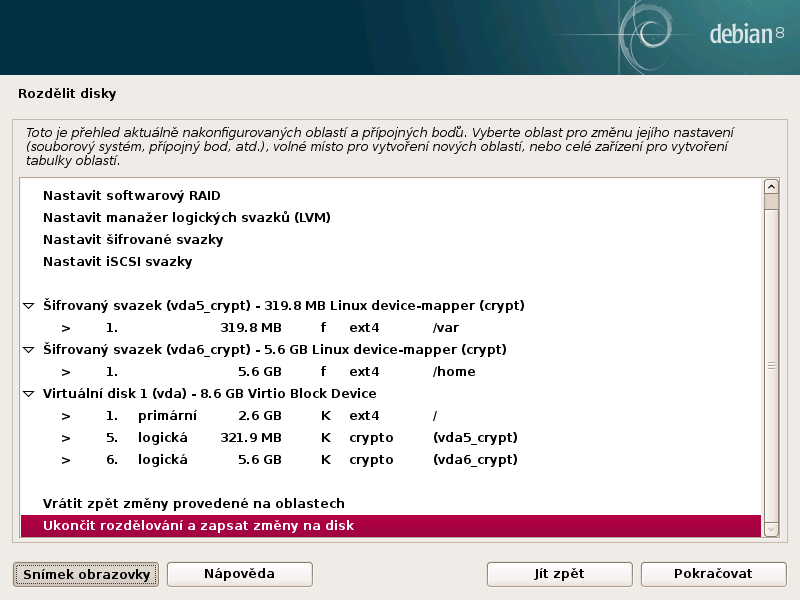
\includegraphics[width=.8\columnwidth]{pictures/debian1.png}
\end{figure}

\subsection{Ubuntu}

	Linux Ubuntu\cite{ubuntu} vychází z~výše zmíněné distribuce Debian, používá však svůj vlastní instalátor. Je také jediným zástupcem linuxové distribuce, která využívá  schéma 
	pro znázornění stavu rozděleného disku. Dříve využívané schéma programu GParted, které detailně rozebírám dále, bylo nahrazeno jednoduchou linkou v~horní oblasti okna instalátoru. Na této lince 
	jsou barevně znázorněny diskové 
	oddíly vytvořené uživatelem. Stejné barvy jsou poté použity u~každého ze záznamů v~seznamu oddílů, jak je možné vidět na obrázku č.~2.2. Tento jednoduchý diagram umožňuje rychlý odhad poměrů různých 
	částí, které budou vytvořeny.

\begin{figure}[h!]
	\label{fig:ubuntu}
	\caption{Distribuce Ubuntu}
	\centering
	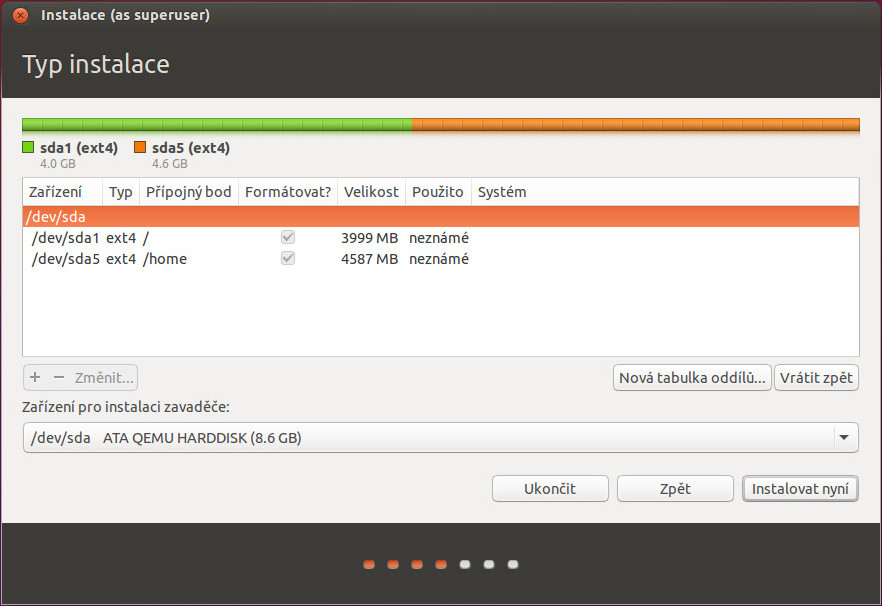
\includegraphics[width=.8\columnwidth]{pictures/ubuntu1.jpg}
\end{figure}

\subsection{CentOS}

	Jako příklad systémů, které využívají instalátor Anaconda, jsem vybral systém CentOS, Community ENterprise Operating System. Na svých stránkách uvádějí: \uv{The CentOS Linux
	distribution is a~stable, predictable, manageable and reproducible platform derived from the sources of Red Hat Enterprise Linux (RHEL).}\cite{centos}. Jedná se v~podstatě o~systém 
	RHEL, ovšem bez podpory a~oprav od společnosti Red Hat. V~současné době instalátor Anaconda používá také pouze textovou reprezentaci rozdělení blokových zařízení. 
	Rozdíl oproti ostatním distribucím tvoří 
	seznam změn, který je zobrazen před finálním potvrzením a~započetím formátování. Na obrázku č.~2.3 můžeme vidět příklad tohoto seznamu. Situaci zpřehledňuje ale pouze pro malý počet změn, seznam s~mnoha 
	záznamy o~změnách je nepřehledný. 

\begin{figure}[h!]
	\label{fig:centos2}
	\caption{Distribuce CentOS příklad souhrné tabulky}
	\centering
	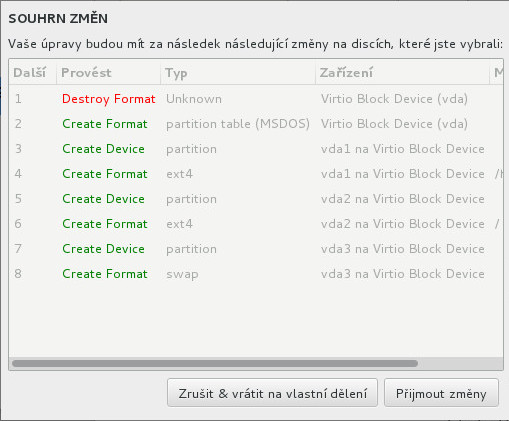
\includegraphics[width=.8\columnwidth]{pictures/centos3.jpg}
\end{figure}

\pagebreak
\subsection{Windows 10}

	Pro srovnání uvádím i~příklad nejrozšířenějšího systému, MS Windows. Vybral jsem v~současnosti nejnovější verzi, Windows 10. Překvapivě ani zde nejsou využity vizuální pomůcky\cite{windows}.
	Tvůrci instalátoru spoléhají na automatickou instalaci a~rozdělení disku s~tím, že pokročilou verzi s~manuálním nastavováním zvolí uživatel, který se zorientuje během instalace i~bez grafické nápovědy. 
	Jak můžeme vidět na obrázku č. 2.4 systém Windows využívá stejný systém jako má distribuce Debian, tj. seznam disků a~jejich oddílů.

\begin{figure}[h!]
	\label{fig:win}
	\caption{Systém Windows}
	\centering
	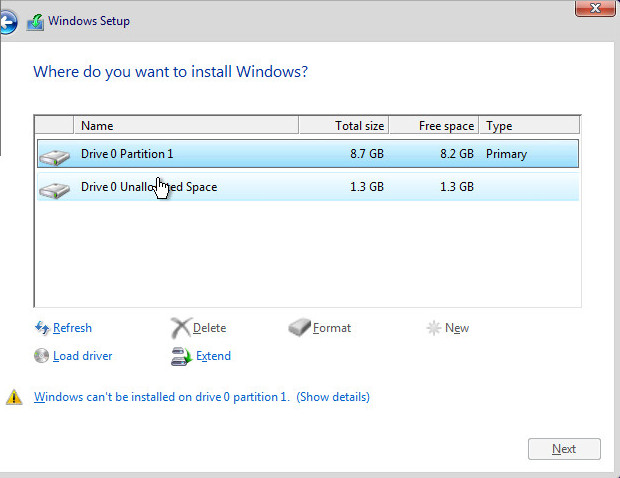
\includegraphics[width=.8\columnwidth]{pictures/win1.jpg}
\end{figure}

\pagebreak
\section{Programy sloužící pro manipulaci se zařízeními}

\subsection{GParted}
	Program GParted\cite{GParted} je zástupcem programů, které je možné spouštět i~mimo fázi instalace systému. S~jeho pomocí lze 
	zvětšovat úložnou kapacitu virtuálních blokových zařízení či disků, jejichž souborový systém umožňuje pozdější modifikaci. Opět je využito dříve zmíněné schéma obdélníku. Každé zařízení je reprezentované
	obdélníkem a~další informace jsou zobrazovány barevnými rámci uvnitř těchto obdélníků. Stejně jak Blivet-gui (zmíněno dále) obsahuje GParted i~grafické aplikace pro manipulaci s~disky 
	a~tím dosahuje efektu WYSIWYG editoru (What You See Is What You Get, editor, který přímo ukazuje aktuální změny). Příkladem je aplikace pro zvětšení diskového oddílu, kterou vidíme na obrázku č.~2.5.

 \begin{figure}[h!]
	 \label{fig:gparted}
	 \caption{Ukázka widgetu pro program GParted~\cite{GParted}}
	 \centering
	 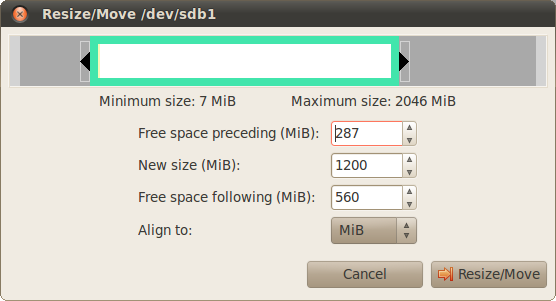
\includegraphics[width=.8\columnwidth]{pictures/gparted-5-big.png}\\
 \end{figure}
 
 \pagebreak
 \subsection{Blivet-gui}

 Druhým příkladem je modul knihovny Blivet, který přidává grafické uživatelké rozhraní. Modul Blivet-gui je dostupný ve všech systémech vycházejících ze systému RHEL. Autoři 
 se zprvu rozhodli použít podobné schéma jako používají ostatní programy, avšak brzy narazili na problém s~větším počtem zařízení včetně virtuálních. Na obrázku č.~2.6 vidíme, že současné řešení je nedostatečné, jednotlivé úrovně 
 barevných rámců 
 jsou znázorněny samostatnými uzly grafu s~hranami vyznačujícími vztahy mezi nimi. Mnoho těchto rámců uživatele spíše zmate a~použití grafu by situaci zpřehlednilo.

 \begin{figure}[h]
	 \label{fig:blivet}
	 \caption{Ukázka programu Blivet-gui~\cite{blivet-gui}}
	 \centering
	 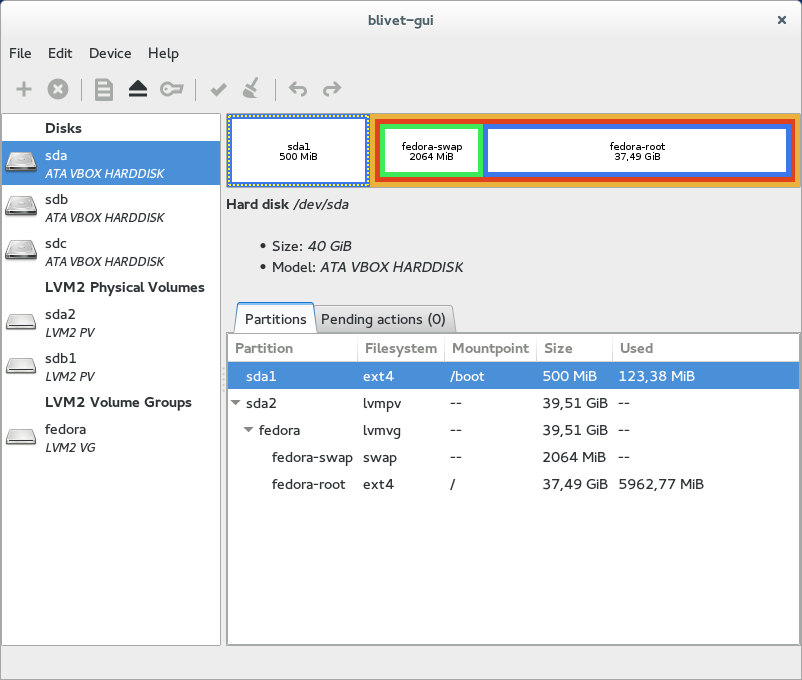
\includegraphics[width=.8\columnwidth]{pictures/blivet-gui-1.png}\\
 \end{figure}

\chapter{Použité knihovny a~technologie}
\section{Knihovna Blivet}
	První a~nejdůležitější knihovou, která je v~mé práci využívána, je knihovna Blivet. Vznikla jako projekt
	ve firmě Red Hat, původně pod jménem pyanaconda.storage\cite{blivet}. Slouží k~rozšíření již zmiňovaného instalátoru Anaconda. Použití této knihovny je součástí zadání, 
	a~proto nebudu diskutovat o~jejích výhodách a~nevýhodách oproti ostatním knihovnám. 

	Mezi její funkce patří i~konfigurace různých datových úložišť, nemusí se jednat pouze o~pevné disky.
	Blivet ovládá i~mnohé další technologie, se kterými se lze v~dnešní době setkat. Příkladem jsou vícenásobná pole nezávislých disků (RAID), technologie logických svazků disku (LVM) či 
	ovládání zašifrovaných modulů pomocí technologie LUKS (Linux Unified Key System, systém pro správu klíčů v~Linuxu). Všechny tři příklady rozebírám níže.

	Dále Blivet obsahuje nástroje pro práci se souborovými systémy diskových oddílů od starších a~již dlouho používaných, jako jsou žurnálovací souborové systémy ext2 až ex4 či ReiserFS\cite{journalFS}  po novější, jako je Btrfs. Také se stará o~bootovací oddíly, čili master boot record (MBR) a~GUID partition table (GPT), tedy o~všechny součásti procesu přípravy úložišť v~rámci instalace nového systému na počítač.

\subsection{RAID}
	Vícenásobná pole nezávislých disků jsou velmi elegantní ochranou před selháním disků. Existůjí různé způsoby, jak pole realizovat, ale základní princip zůstává vždy stejný. 
	Několik disků, vystupuje jako jediný\cite{RAID}. Jedním z~příkladů použití vícenásobného diskového pole může být disk s~kapacitou rovnou součtu disků, ze kterých je tvořen, anebo také
	kapacitou jednoho disku, přičemž data jsou z~něj zrcadlena na ostatní disky. Cílem tohoto nastavení je ochrana před selháním hardwaru a~ztrátou dat. 
	
	Blivet obsahuje nástroje pro práci s~programem mdadm, která slouží k~nastavení softwarového pole RAID. Při využití hardwarových technologií, zvláště pak proprietárních,
	je možné k~tomuto RAIDu přistupovat jako k~obyčejnému disku, čehož i~nesvobodné RAIDy často využívají a~svých mnoho disků skrývají za jednotným rozhraním, které vystupuje jako jeden
	disk. 

	Program mdadm je softwarový RAID, a~proto má počítač celou dobu přehled nejen o~finálním disku zabezpečeném proti selhání, ale i~o~všech dílčích discích, které ho tvoří. Výhodou
	softwarového RAIDu je
	možnost monitorování redundantních disků nástroji, které jsou součástí systému, bez nutnosti využívání aplikace třetích stran, u~kterých hrozí nekompatibilita, případně další 
	komplikace.
	Mezi nevýhody tohoto nastavení se řadí menší přehlednost při práci se všemi disky počítače, kdy změna jednoho disku vyvolá řetězovou reakci dalších změn. Právě proto je třeba data uceleně třídit
	a~pokud možno i~přehledně vizualizovat.

\subsection{LVM}
  LVM neboli Logical Volume Management je metoda, kterou je možné spravovat diskové oddíly. Poskytuje větší flexibilitu volného místa než klasické diskové oddíly a~pracuje se třemi
	úrovněmi
	zařízení\cite{LVM}. První úrovní jsou fyzické svazky neboli physical volumes (PV). Fyzický svazek je tvořen buď samotným diskem, včetně například disku RAID, nebo diskovým oddílem. 
	Fyzické
	svazky nenabízí o~mnoho více funkcionality, než je označení a~příprava svazku pro další práci. Ta spočívá v~rozdělení fyzického svazku na fyzické extenty (physical extents, PE).

	Další úrovní jsou skupiny svazků (volume groups, VG), sdružující jeden nebo více fyzických svazků a~logických svazků (LV). Skupiny svazků disponují úložným prostorem svých PV, 
	který rozdělují mezi LV. Výhodou existence VG je možnost libovolně přidávat svazky, a~to i~za plného chodu systému. Za chodu systému lze místo z~VG i~ubírat, ale 
	pouze dosud neobsazenou část. 

	Třetí úrovní LVM jsou již zmíněné logické svazky, které jsou dostupné uživateli k~ukládání dat. Z~tohoto pohledu se chovají stejně jako obyčejné diskové oddíly. Jak již ale
	bylo zmíněno, výhodou oproti obyčejným diskovým oddílům je flexibilita dostupného místa. Na logických svazcích je možné vytvářet souborové systémy a~dále s~nimi pracovat.

	Kromě úprav velikosti oddílů za chodu je také možné data v~rámci VG přesouvat. LVM také umí vytvářet snímky, tj. zachycovat stav dat v~čase. Využítí nachází tato 
	vlastnost
	při vytváření záloh a~jako záchytný bod, ke kterému je možné se vrátit. Nevýhodou LVM je skutečnost, že data na fyzických svazcích mohou být fragmentována, a~tak
	dochází ke snížení výkonu. Také je třeba mít na zřeteli fakt, že pokud zmenšujeme logický svazek, musí tuto funkci obsahovat i~souborový systém, který se na něm nachází.

\subsection{LUKS}
	Linux Unified Key Setup (unifikované nastavení klíčů na linuxu) je specifikace šifrování blokových zařízení původně vytvořená pro systém Linux. Existují i~implementace na jiné 
	systémy
	těmi se zde ale nezabývám. LUKS vznikl, aby usnadnil proces nastavování šifrovaných dat, slovy autora: \uv{It has initially been developed to remedy the unpleasantness a~user 
	experienced that arise from deriving the encryption setup from changing user space, and forgotten command line arguments. The result of this changes are an unaccessible encryption
	storage.}\cite{on-disk-format} V~současné době se LUKS používá společně s~technologií dm-crypt, která slouží jako prostředek k~šifrování.

	Při využití LUKS v~Blivetu lze šifrovat všechna bloková zařízení (disky, diskové oddíly, logické svazky i~fyzické svazky). Celé nastavení LVM může být šifrováno jedním klíčem, v~současnosti se takto 
	standardně šifruje LVM ve Fedora Linuxu, pokud uživatel nastaví automatické rozdělení zařízení s~šifrováním. Nemusí se jednat jen o~pevné disky, ale také o~odstranitelná média jako
	SD karty nebo USB paměti. Šifrovat lze též odkládací prostor paměti (swap).

\subsection{Formáty souborového systému}
  Jak již bylo zmíněno, Blivet umí pracovat i~se souborovými systémy. Struktura je následující: Výchozí seznam zařízení reprezentující jednotlivé disky, jejich oddíly a~případně
	speciální technologie jako RAID, LVM či šifrování LUKS. Každé zařízení má ale možnost mít i~formát, čímž se myslí formát souborového systému. Podporována je většina známých 
	souborových
	systémů. Patří mezi ně souborový systém ext, ReiserFS, XFS. Taktéž existuje podpora pro Btrfs (B-tree FS)\cite{btrfs}, experimentální souborový systém 
	společnosti Oracle. Přestože zatím u~Btrfs neexistuje stabilní verze, je mezi distribucemi podporován, neboť nabízí řešení některých problémů současných souborových systémů.

\section{Graphviz}
	Graphviz je program, který slouží k~vizualizaci dat formou orientovaných či neorientovaných grafů\cite{graphviz}. Pomocí Graphvizu je možné generovat grafy sloužící ke znázornění počítačové sítě nebo
	vztahů mezi určitými objekty. Nelze vytvářet grafy průběhů funkcí či grafy znázorňující vztahy mezi číselnými hodnotami. Jinými slovy Graphviz generuje grafy, jaké známe z~teorie grafů,
	ale není schopen generovat grafy známé například z~ekonomie.

	Program je z~velké části napsán v~jazyce C, ale ve existují obalovací knihovny (wrapper libraries) pro mnoho výšších programovacích jazyků. Vyššími 
	programovacími jazyky myslím jazyky, které jsou pokládány za méně náročné na obstarávání systémových věcí programátorem. Typickým příkladem výššího 
	programovacího jazyka je jazyk Java. Dalšímy příklady je Python a~PHP. Často jsou tyto jazyky označovány jako skriptovací. 
	Z~těchto knihoven se budeme soustředit hlavně na knihovnu pro Python 3, která je používána v~mé práci.

	Hlavními elementy při vytváření grafu jsou graf (graph), uzel (node) a~hrana (edge). Základní grafy lze tvořit jen pomocí těchto tří klíčových slov.

\subsection{Graf}
	Klíčové slovo graph uvádí jakýkoliv graf, který bude vytvořen, včetně prvního kořenového grafu. Každý zápis v~jazyce DOT musí začínat slovem graph nebo digraph\cite{digraph}. Výjimku tvoří užití slova
	strict, které se uvádí na začátku zápisu a~které zamezuje vzniku vícenásobných hran tedy působí, že  mezi každým počátečním a~koncovým uzlem bude jen jedna hrana. 

	Graph označuje graf neorientovaný. Slovo digraph je zkrácené spojení directed graph (orientovaný
	graf) a~vyjadřuje graf orientovaný. Při vizualizaci rozdělení diskového prostoru jsem se rozhodl použít právě orientované grafy, neboť považuji za 
	důležité poskytnout uživateli co nejvíce vodítek ke znázornění vztahu rodič~-~potomek a~orientované hrany jsou ideální pro tento účel. 

	Speciálním případem grafu je podgraf (subgraph). Grafy mohou být vkládány do sebe a~pomocí podgrafů lze snížit velikost zdrojového kódu v~jazyce DOT. Příkladem budiž situace, kdy zápisem
	hrany vedoucí od uzlu k~podgrafu (\texttt{A~--~\{B C\}}) vytvoříme stejný efekt jako při zápisu každé jednotlivé dvojice mezi uzlem A~a~uzly B a~C (\texttt{A~--~B, A~--~C}). Dále je možné podgrafy využít
	pro specifikaci odlišných atributů uzlů či hran. V~podgrafu lze jednoduše nastavit jiné atributy než ve zbytku grafu.

	Poslední situací pro využití podgrafu je situace, kdy chceme uzly shlukovat. V~tomto případě je nutné přidat k~názvu podgrafu klíčové slovo cluster a~určité grafovací algoritmy tyto uzly 
	uspořádají k~sobě do skupiny.

\subsection{Uzly}
	Uzly jsou základem každého grafu. V~Graphvizu jsou definovány svým jménem. Základní graf s~jedním uzlem definujeme v~jazyce DOT jednoduše, a~to: \texttt{graf \{A\}}. Tento zápis vytvoří
	graf s~jedním uzlem uprostřed. Ve středu grafu bude napsán název uzlu. Uzly mají mnoho různých atributů od svého jména po URL odkazy a~atributy HTML formátování. 
	Nejdůležitějšími jsou ty, které jsou definovány v~základním nastavení. Jsou to tvar uzlu (shape), barva výplně (fillcolor) a~jméno (name) nebo štítek (label). 
	
	Standardně je tvar nastaven na elipsu a~barva
	na bílou. Jméno se bere podle identifikátoru při vytváření uzlu, štítek je rozšířením jména. Pokud je definován, štítek nahrazuje jméno a~její obsah je vepsán dovnitř uzlu. Od jména se liší 
	tím, že její obsah lze libovolně upravovat, avšak lze do ní ukládat pouze text, jakékoliv speciální formátování nebude zohledněno. Pro vkládání obrázků slouží atribut image a~pro vkládání
	odkazů atribut url.

	Právě třemi základními atributy jsem se rozhodl rozlišovat jednotlivé typy zařízení, se kterými pracuje Blivet. Pomocí tvaru uzlu odlišuji technologie zařízení. Čím je technologie
	abstraktnější, tím zaoblenější tvar má. Pevné disky a~jejich oddíly jsou znázorněny čtverci, LVM čtverci se zaoblenými rohy a~zařízení připojené přes síť či šifrování jsou znázorněny elipsou.
	Pro toto dělení jsem se rozhodl, abych zachoval konzistenci celého grafu a~pomohl uživateli rozlišit rozdíly jen pomocí krátkého zhlédnutí tvaru.

	Druhým odlišovacím prvkem je barva, a~to jak její odstín, tak sytost. Některé odstíny jsou rezervovány pro odlišení akcí, které budou provedeny při konfiguraci. Zelenou barvou jsou vyznačeny
	nově se objevivší prvky, červenou zaniknuvší prvky a~oranžovou prvky, u~kterých došlo ke změnám. Sytost barvy společně s~tvarem jasně definují použitou technologii. Barva pomáhá tam, kde
	samotný tvar nestačí. Čili pokud používá stejný tvar jak šifrování, tak blokové zařízení připojené přes internet, dojde k~jejich jednoznačnému odlišení použitím sytější a~méně syté barvy.

\subsection{Hrany}
	Hrany nejsou tak komplikovanými elementy jako uzly. Jejich základní atributy jsou počáteční a~koncový uzel. U~neorientovaného grafu se nerozlišuje, který uzel je počáteční. Hrany 
	nepoužívají tolik atributů jako uzly, avšak například štítek stále mít mohou. Vzhledem k~jejich tvaru je u~nich zbytečný atribut výplňové barvy (fillcolor) a~používá se jen barva 
	\uv{pera}.
	Jak již bylo zmíněno, v~mé praci jsou všechny grafy orientované, a~tak záleží na pořadí v~jakém jsou uzly předány funkci, která tvoří hrany. Nicméně směr je vždy od rodiče k~potomkovi
	a~nikdy naopak.
	
\subsection{Rozložení}
	Graphviz nabízí různé možnosti rozložení grafu. Základních je pět, dot, neato, fdp, twopi, circo. Ke každému rozložení přikládám obrázek a~rozebírám jej 
	podrobněji. U~každého příkladu je použit stejný vstupní zápis, ale výsledky se velmi liší. Vstupní data vypadají takto:
	\pagebreak[4]
	\begin{quotation}
		\texttt{graph\{\\
		A~-- B\\
		B -- C\\
		C -- D\\
		D -- A\\
		D -- E\\
		D -- F\\
		G -- B\\
		G -- E\\
	\}}
	\end{quotation}

	Prvním rozložením je rozložení dot. Oficiální dokumentace k~němu říká:
	\uv{dot -- 'hierarchical' or layered drawings of directed graphs. This is the default tool to use if edges have directionality.}\cite{graphviz_layout} 
	Rozhraní dot přehledně udržuje hierarchii mezi rodiči a~potomky. Skládá
	své uzly do stromu, a~proto by mohl být kandidátem na použití v~mé práci. Lidé jsou zvyklí vnímat data ohledně úložného prostoru ve formě stromů. Tím pádem jde o~intiutivnější
	reprezentaci.

\begin{figure}[h!]
	\label{fig:Ukázka rozložení dot}
	\caption{Ukázka rozložení dot}
	\centering
	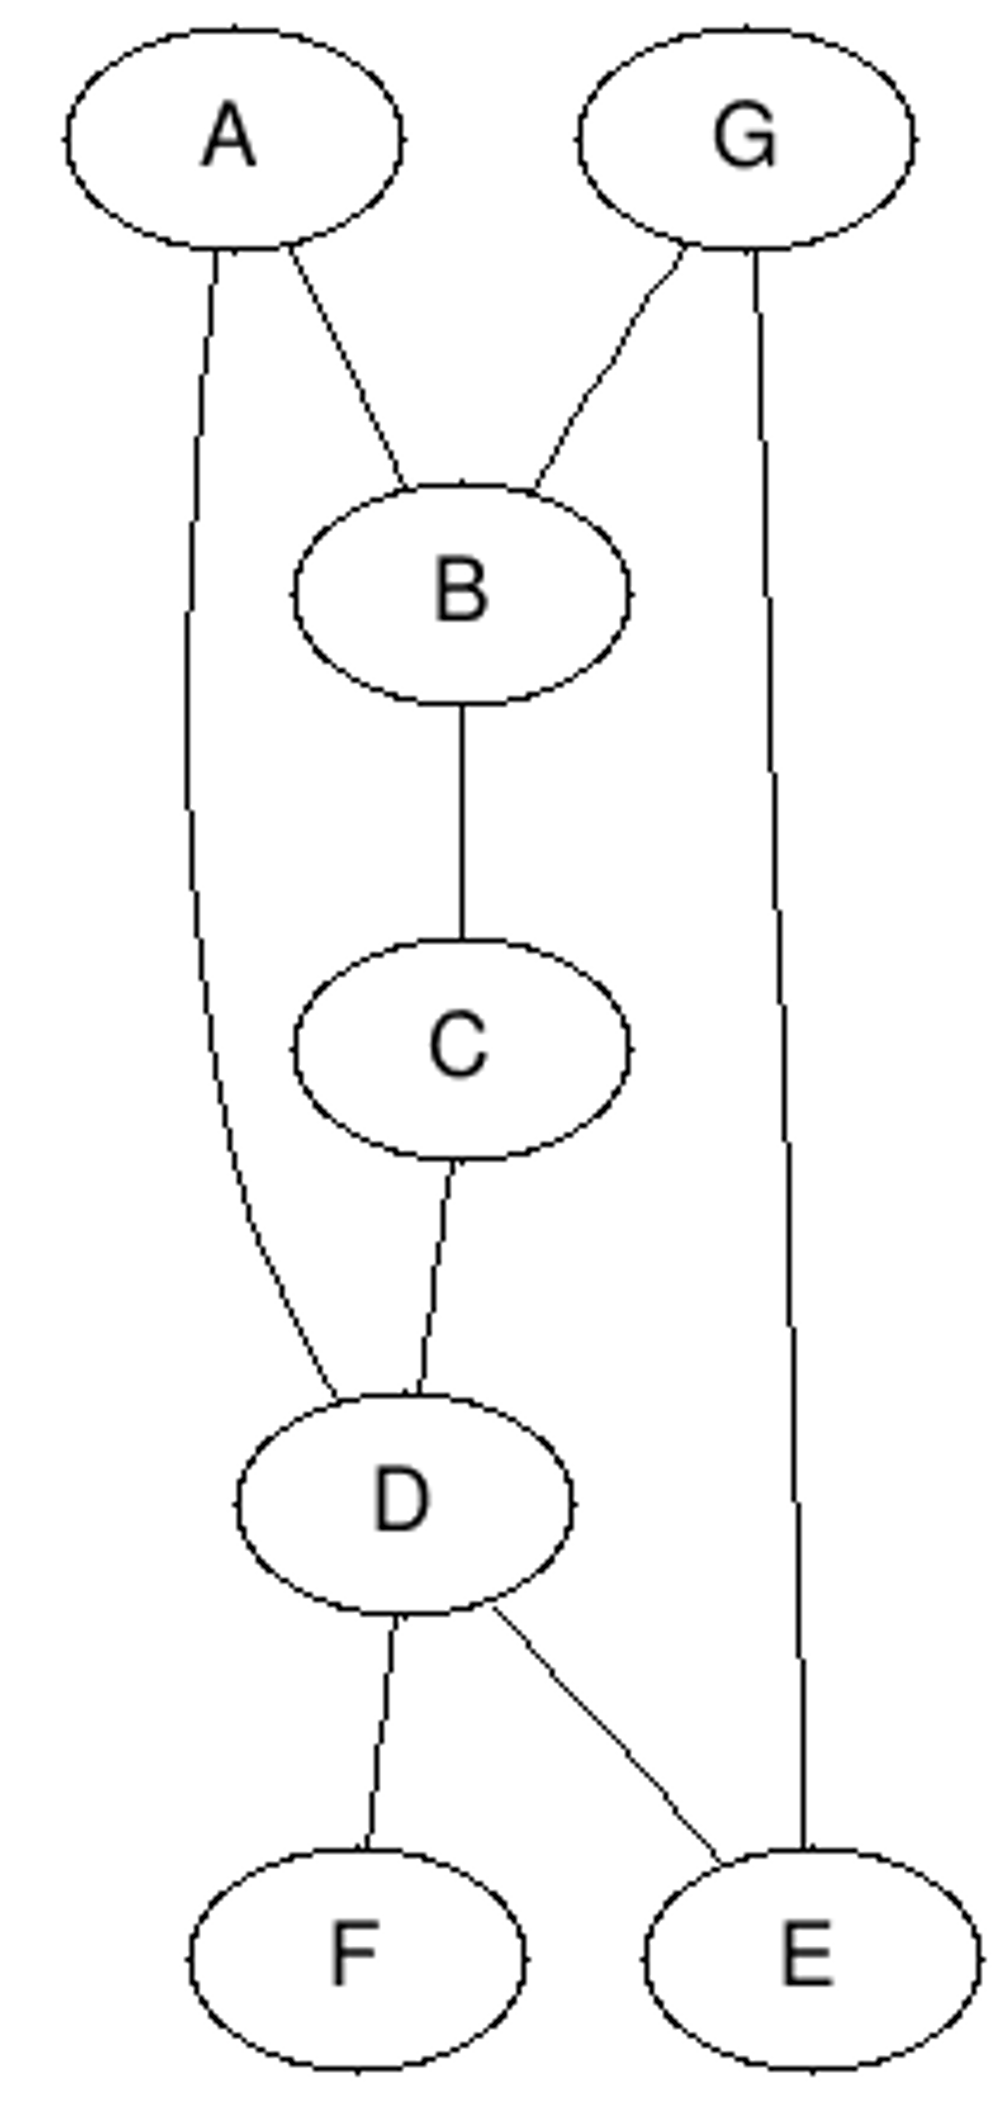
\includegraphics[width=0.4\textwidth]{pictures/dot_example.png} 
\end{figure}

	Druhé rozložení, \uv{neato -- 'spring model' layouts.  This is the default tool to use if the graph is not too large (about 100 nodes) and you don't know anything else about it. Neato attempts to
	minimize a~global energy function, which is equivalent to statistical multi-dimensional scaling.}\cite{graphviz_layout}
	Jinými slovy algoritmus neato se snaží vytvořit celý graf co nejmenší bez ohledu na ostatní faktory. Grafy nejsou hierarchické ani 
	strukturované. Cílem je co nejmenší zabraná plocha a~zároveň nepřekrývání hran a~uzlů. Kvůli chaotičnosti a~nestrukturalizovanosti se nejedná o~algoritmus který, bych mohl
	použít. Ostatně neato je přizpůsobeno na neorinetované grafy.

\begin{figure}[h!]
	\label{fig:Ukázka rozložení neato}
	\caption{Ukázka rozložení neato}
	\centering
	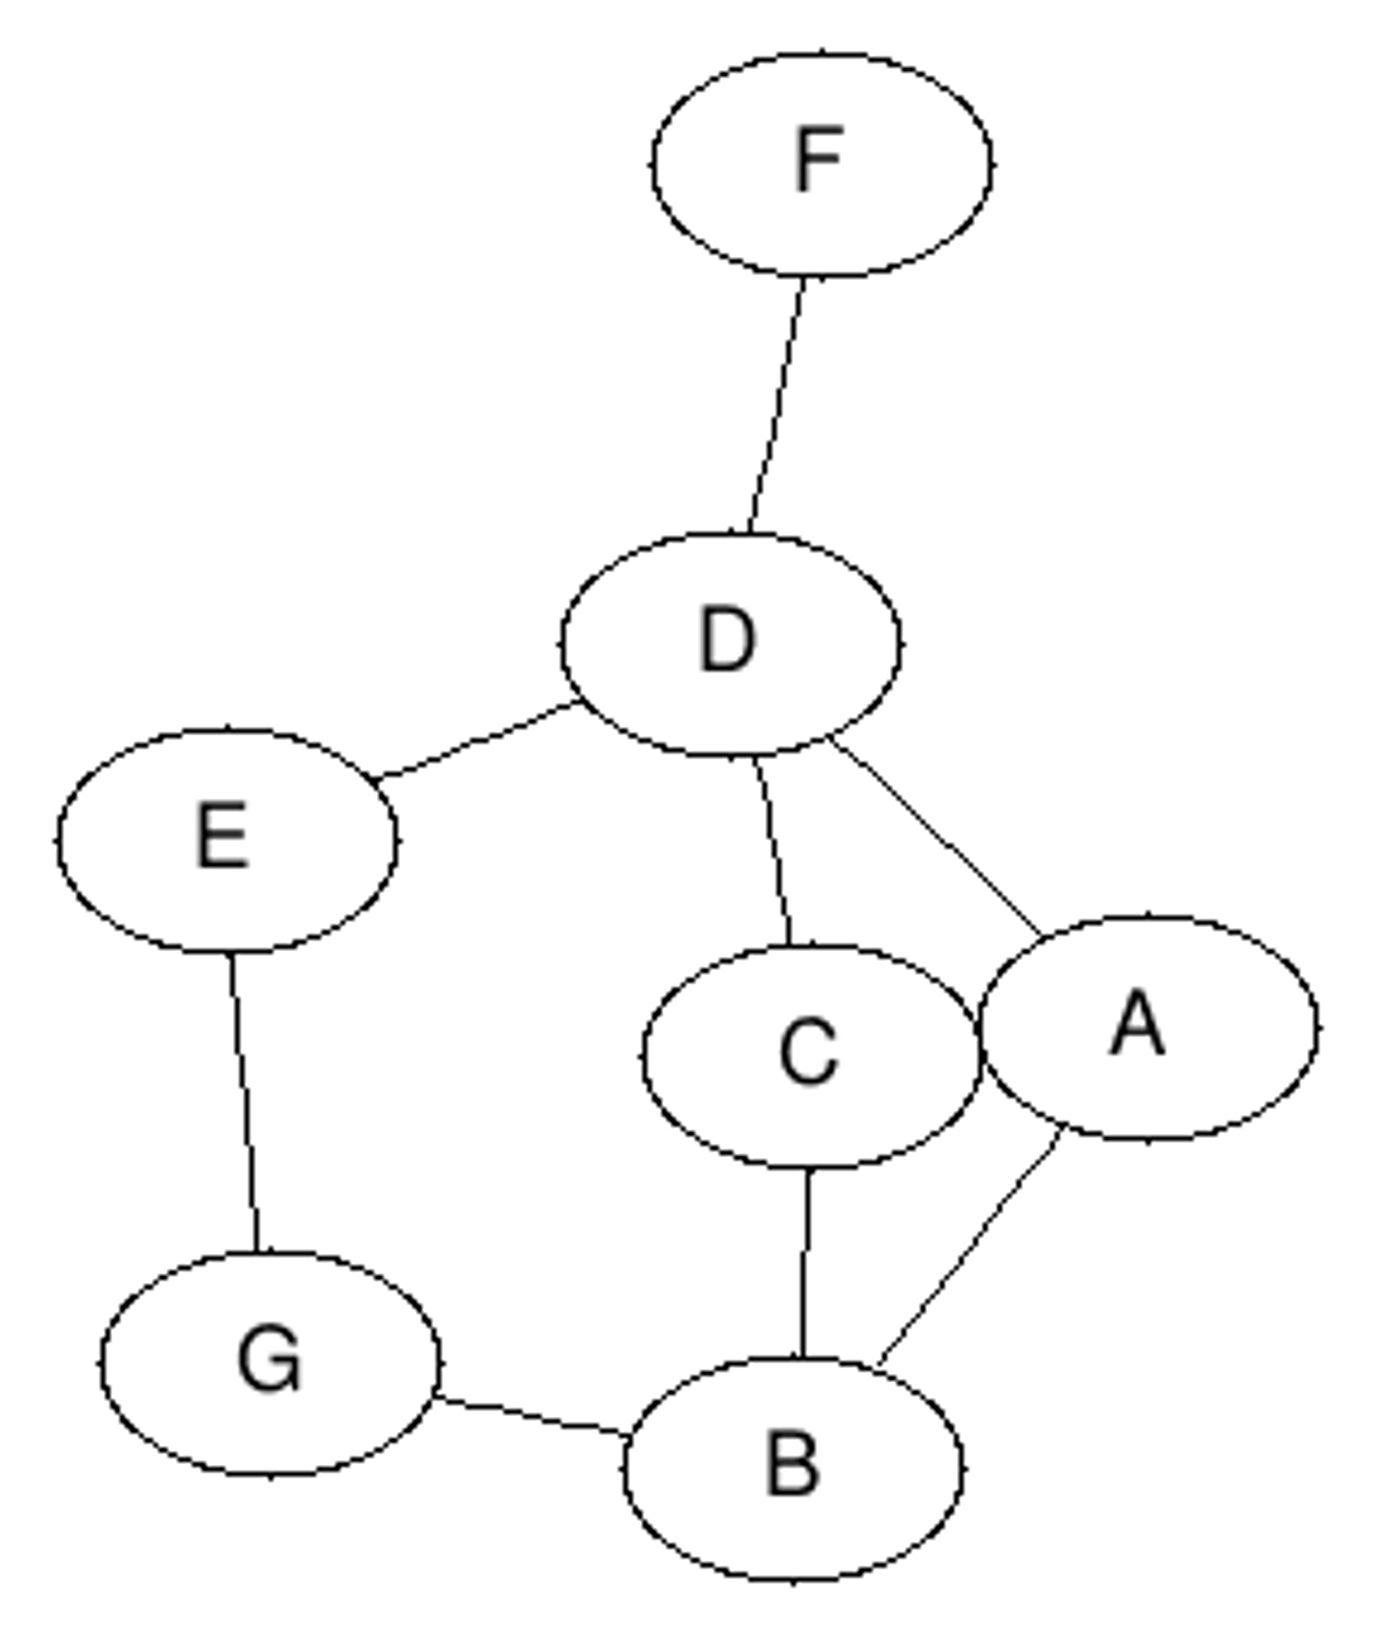
\includegraphics[width=0.6\textwidth]{pictures/neato_example.png} 
\end{figure}

	Třetí rozložení, \uv{fdp -- 'spring model' layouts similar to those of neato, but does this by reducing forces rather than working with energy.}\cite{graphviz_layout} 
	Fdp je další z~rozložení pro neorientované grafy, ještě více zmenšuje plochu grafu, tentokrát i~s~ústupkem ohledně překrývání
	uzlů hranami. Pro grafy, které potřebuji vytvořit, se jedná o~ten nejhorší algoritmus z~pěti zde zmíněných. V~uzlech jsou zapsána data o~zařízeních a~hrany překrývající tyto uzly
	působí rušivě. Zároveň není třeba šetřit místem, neboť ve výsledné aplikaci je možné přibližovat a~posouvat graf dle libosti uživatele. Fpd tedy není algoritmem vhodným pro tuto
	situaci.

\begin{figure}[h!]
	\label{fig:Ukázka rozložení fdp}
	\caption{Ukázka rozložení fdp}
	\centering
	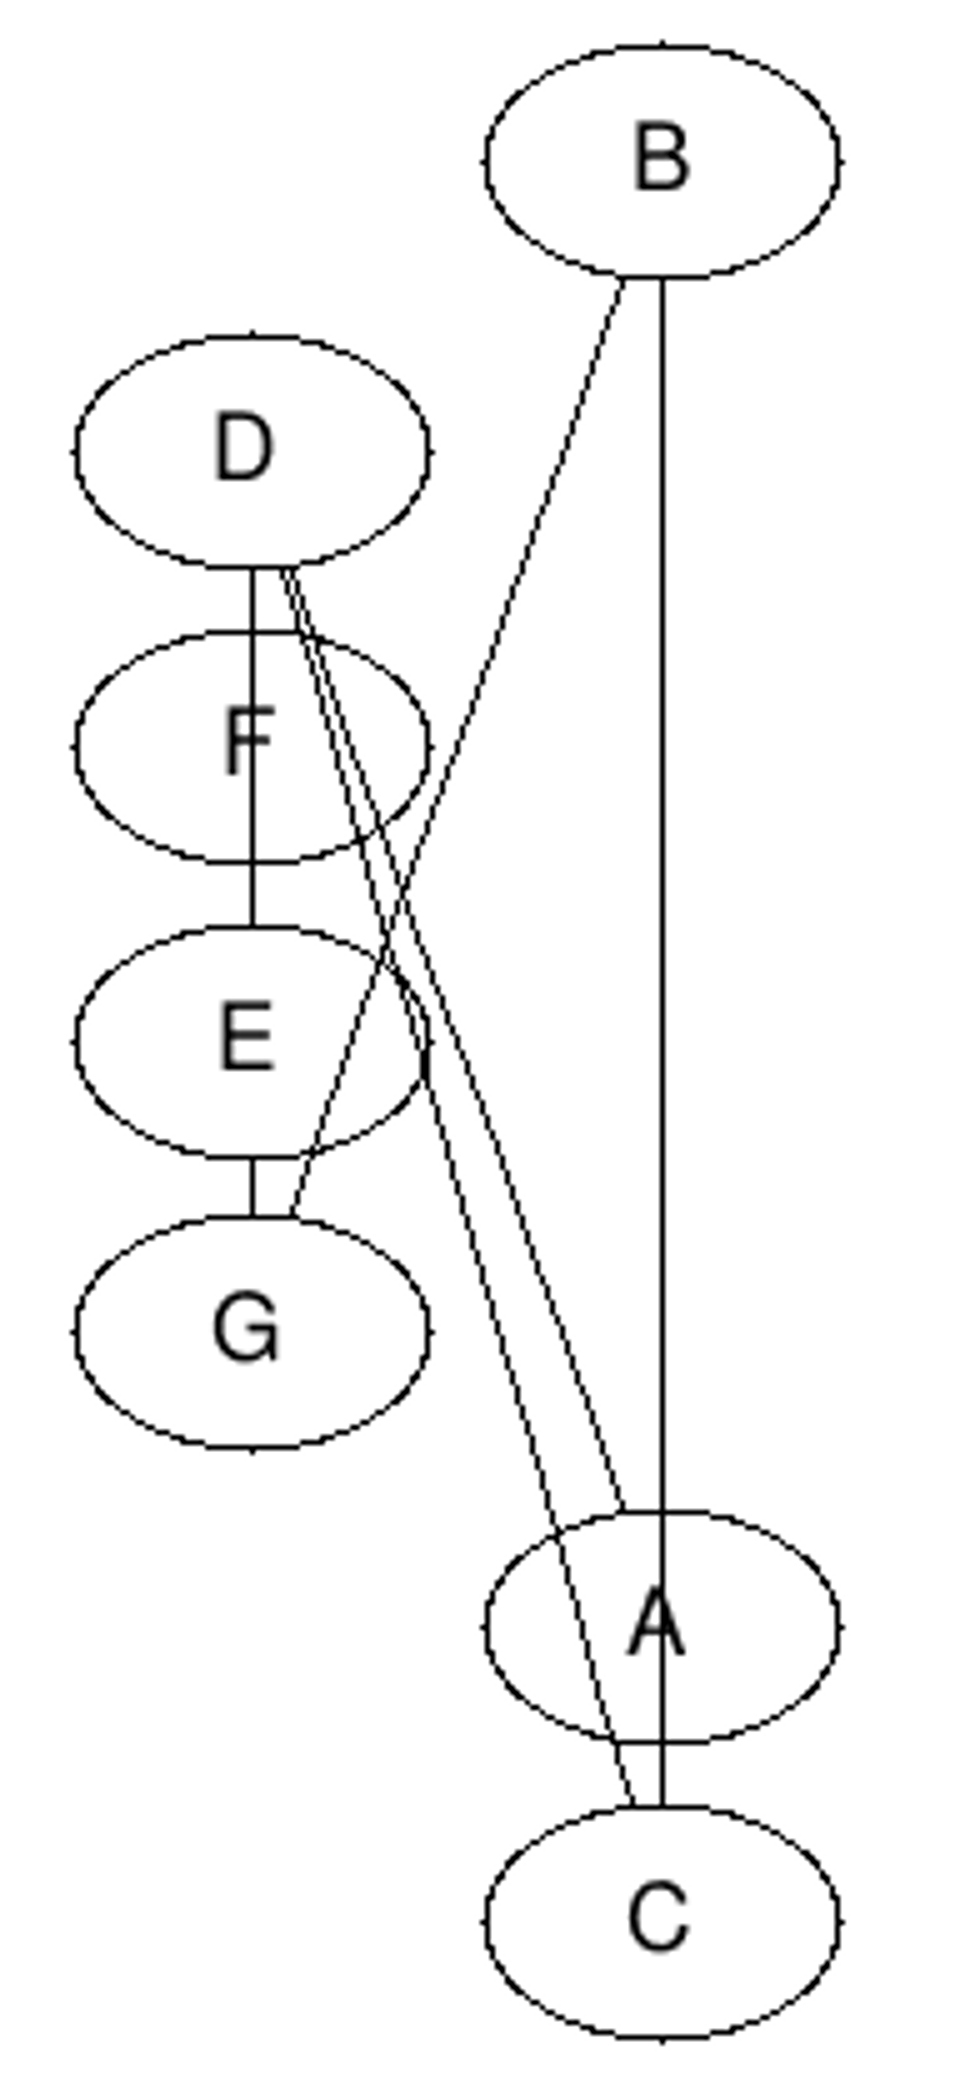
\includegraphics[width=0.4\textwidth]{pictures/fdp_example.png} 
\end{figure}

	Čtvrté rozložení, \uv{twopi -- radial layouts.  Nodes are placed on concentric circles depending their distance from a~given root node.}\cite{graphviz_layout}
	Použitím paprskového rozložení dochází k~strukturalizaci grafu, tím pádem by se algoritmus twopi mohl zdát 
	dobrou volbou pro uskutečnění cíle, který jsem si vytyčil. Ovšem přidáním dalších dvou uzlů, které způsobí rozvětvení grafu, se strukturalizace začne vyvíjet neakceptovatelným směrem.
	Oba případy jsou vidět na obrázcích č.~3.4 a~3.5. Strukturovanost do kruhů by, dle mého názoru, uživatele zbytečně mátla. Je důležité mít kořenový uzel, ovšem jeho umístění doprostřed je špatnou
	volbou.

\begin{figure}[h!]
	\label{fig:Ukázka rozložení twopi}
	\caption{Ukázka rozložení twopi}
	\centering
	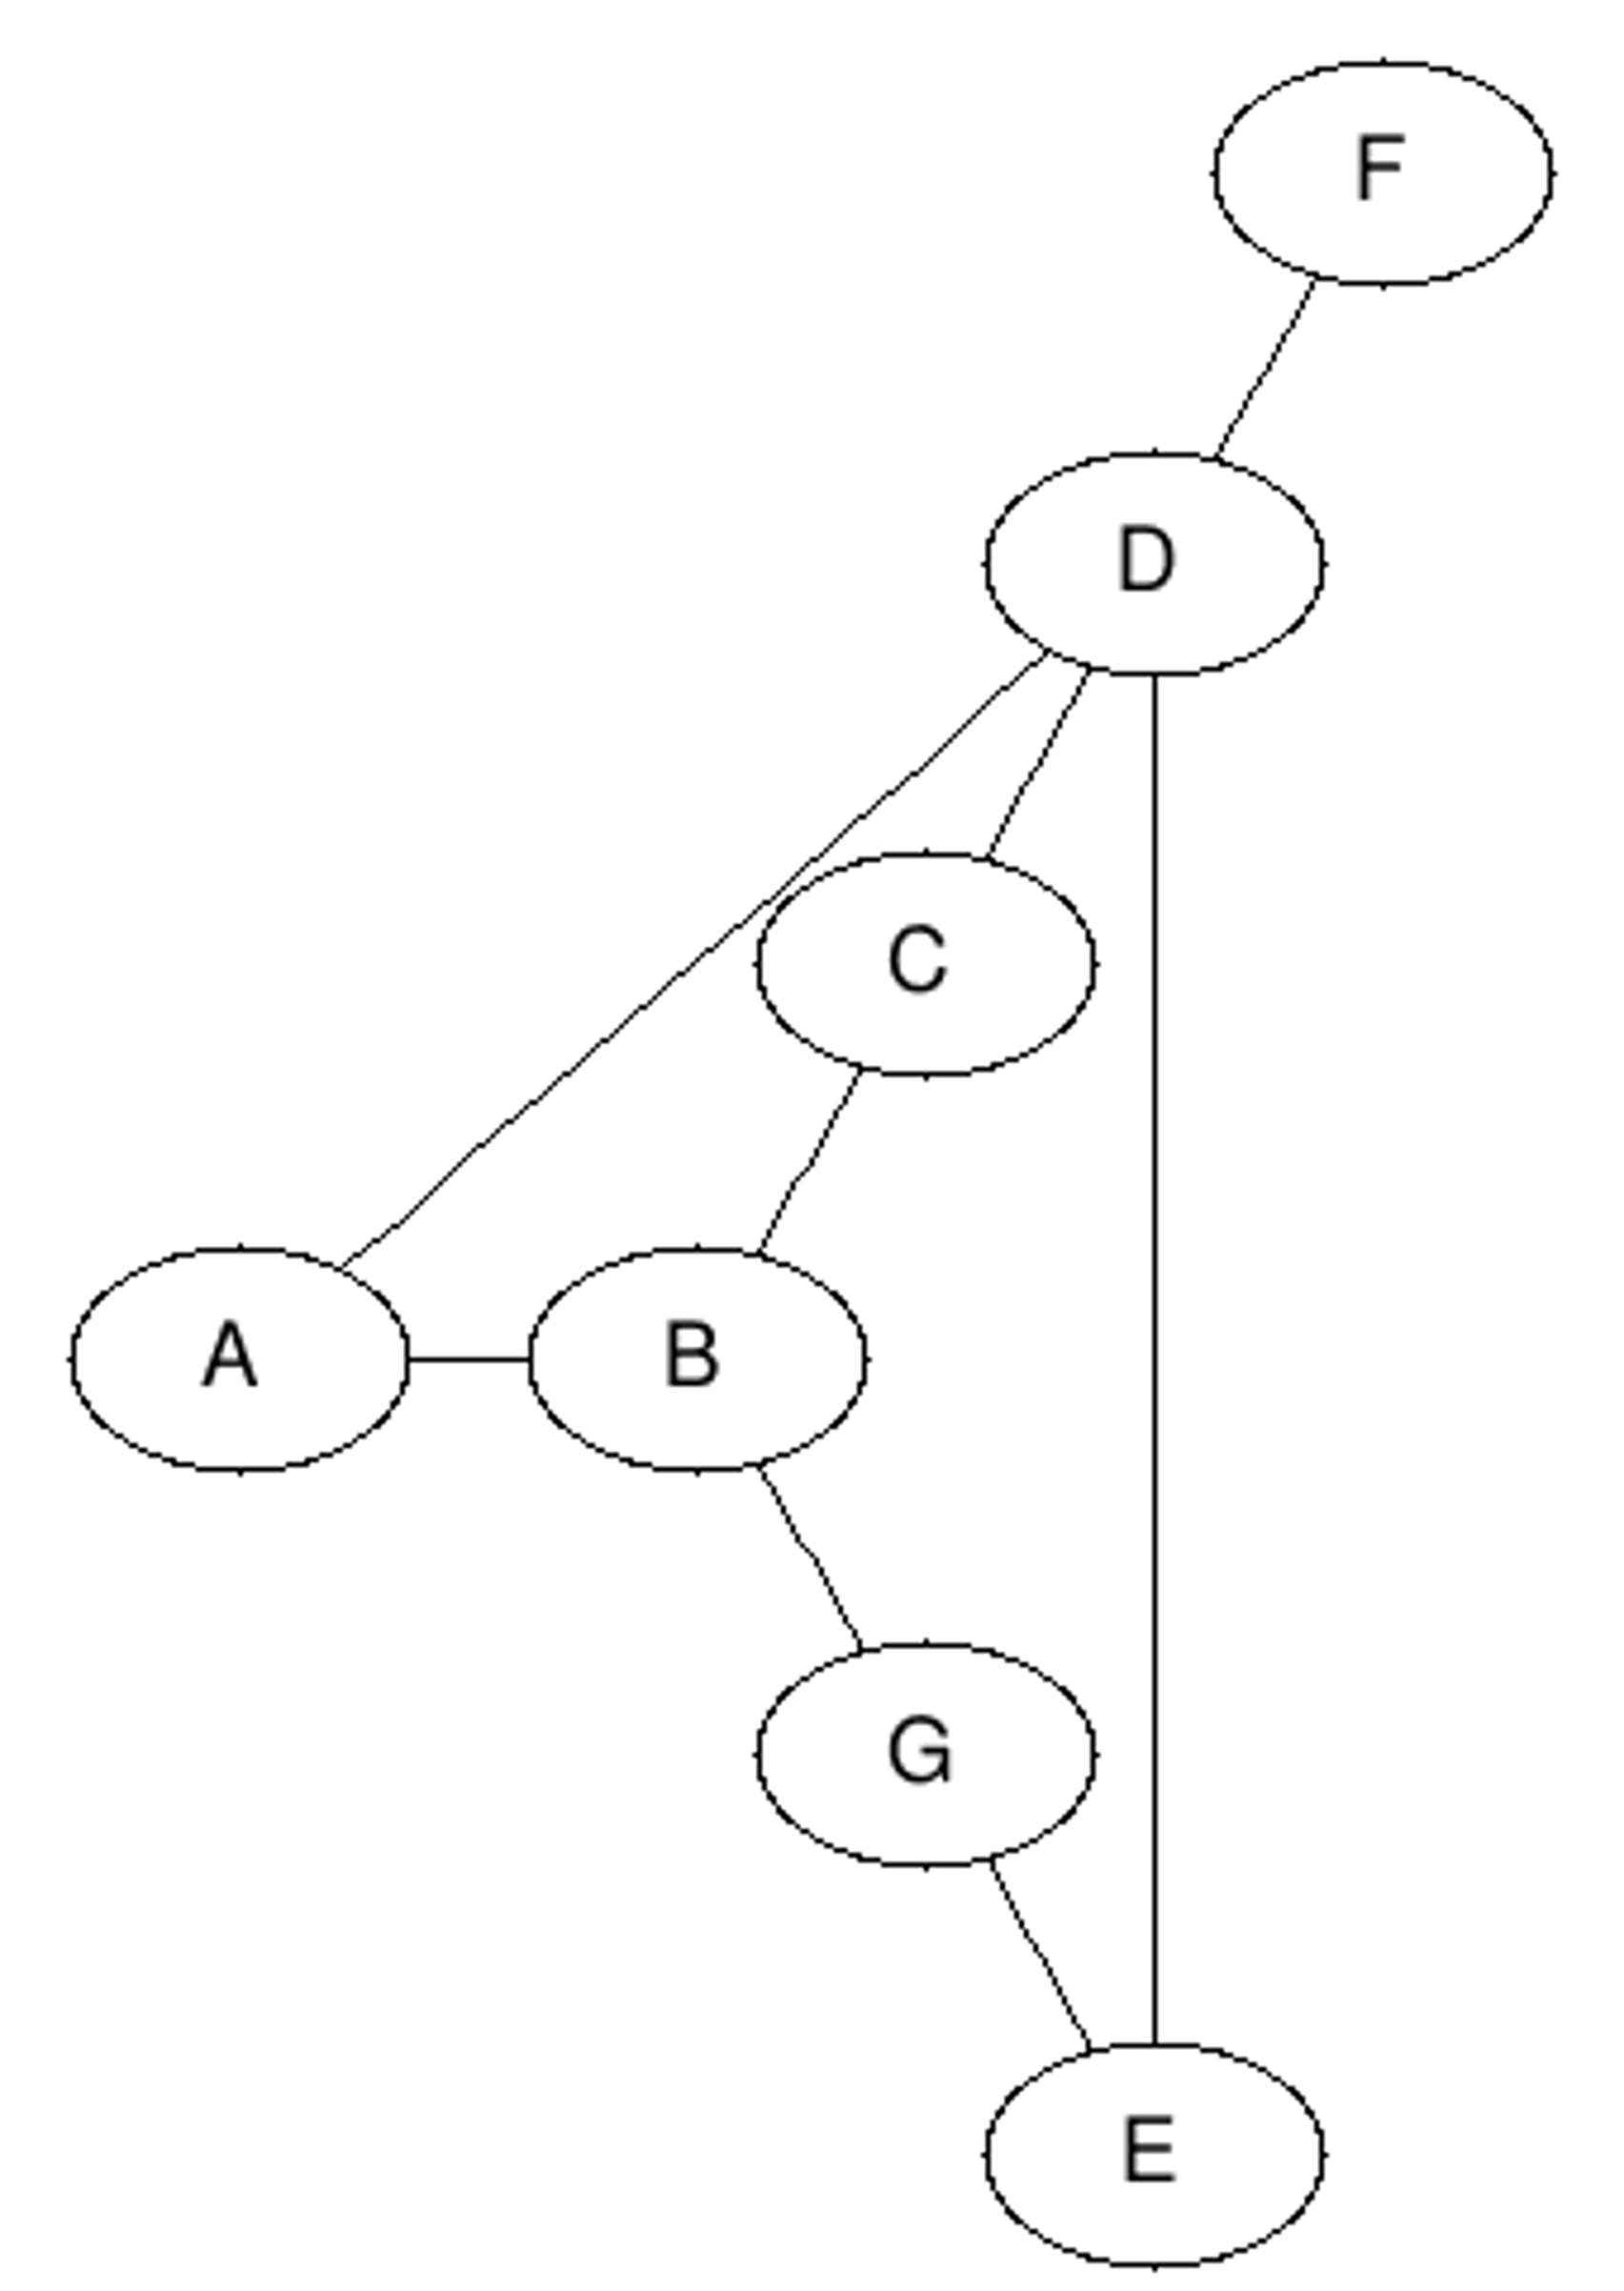
\includegraphics[width=0.6\textwidth]{pictures/twopi_example.png} 
\end{figure}
\begin{figure}
	\label{fig:Ukázka rozložení twopi}
	\caption{Druhá ukázka rozložení twopi}
	\centering
	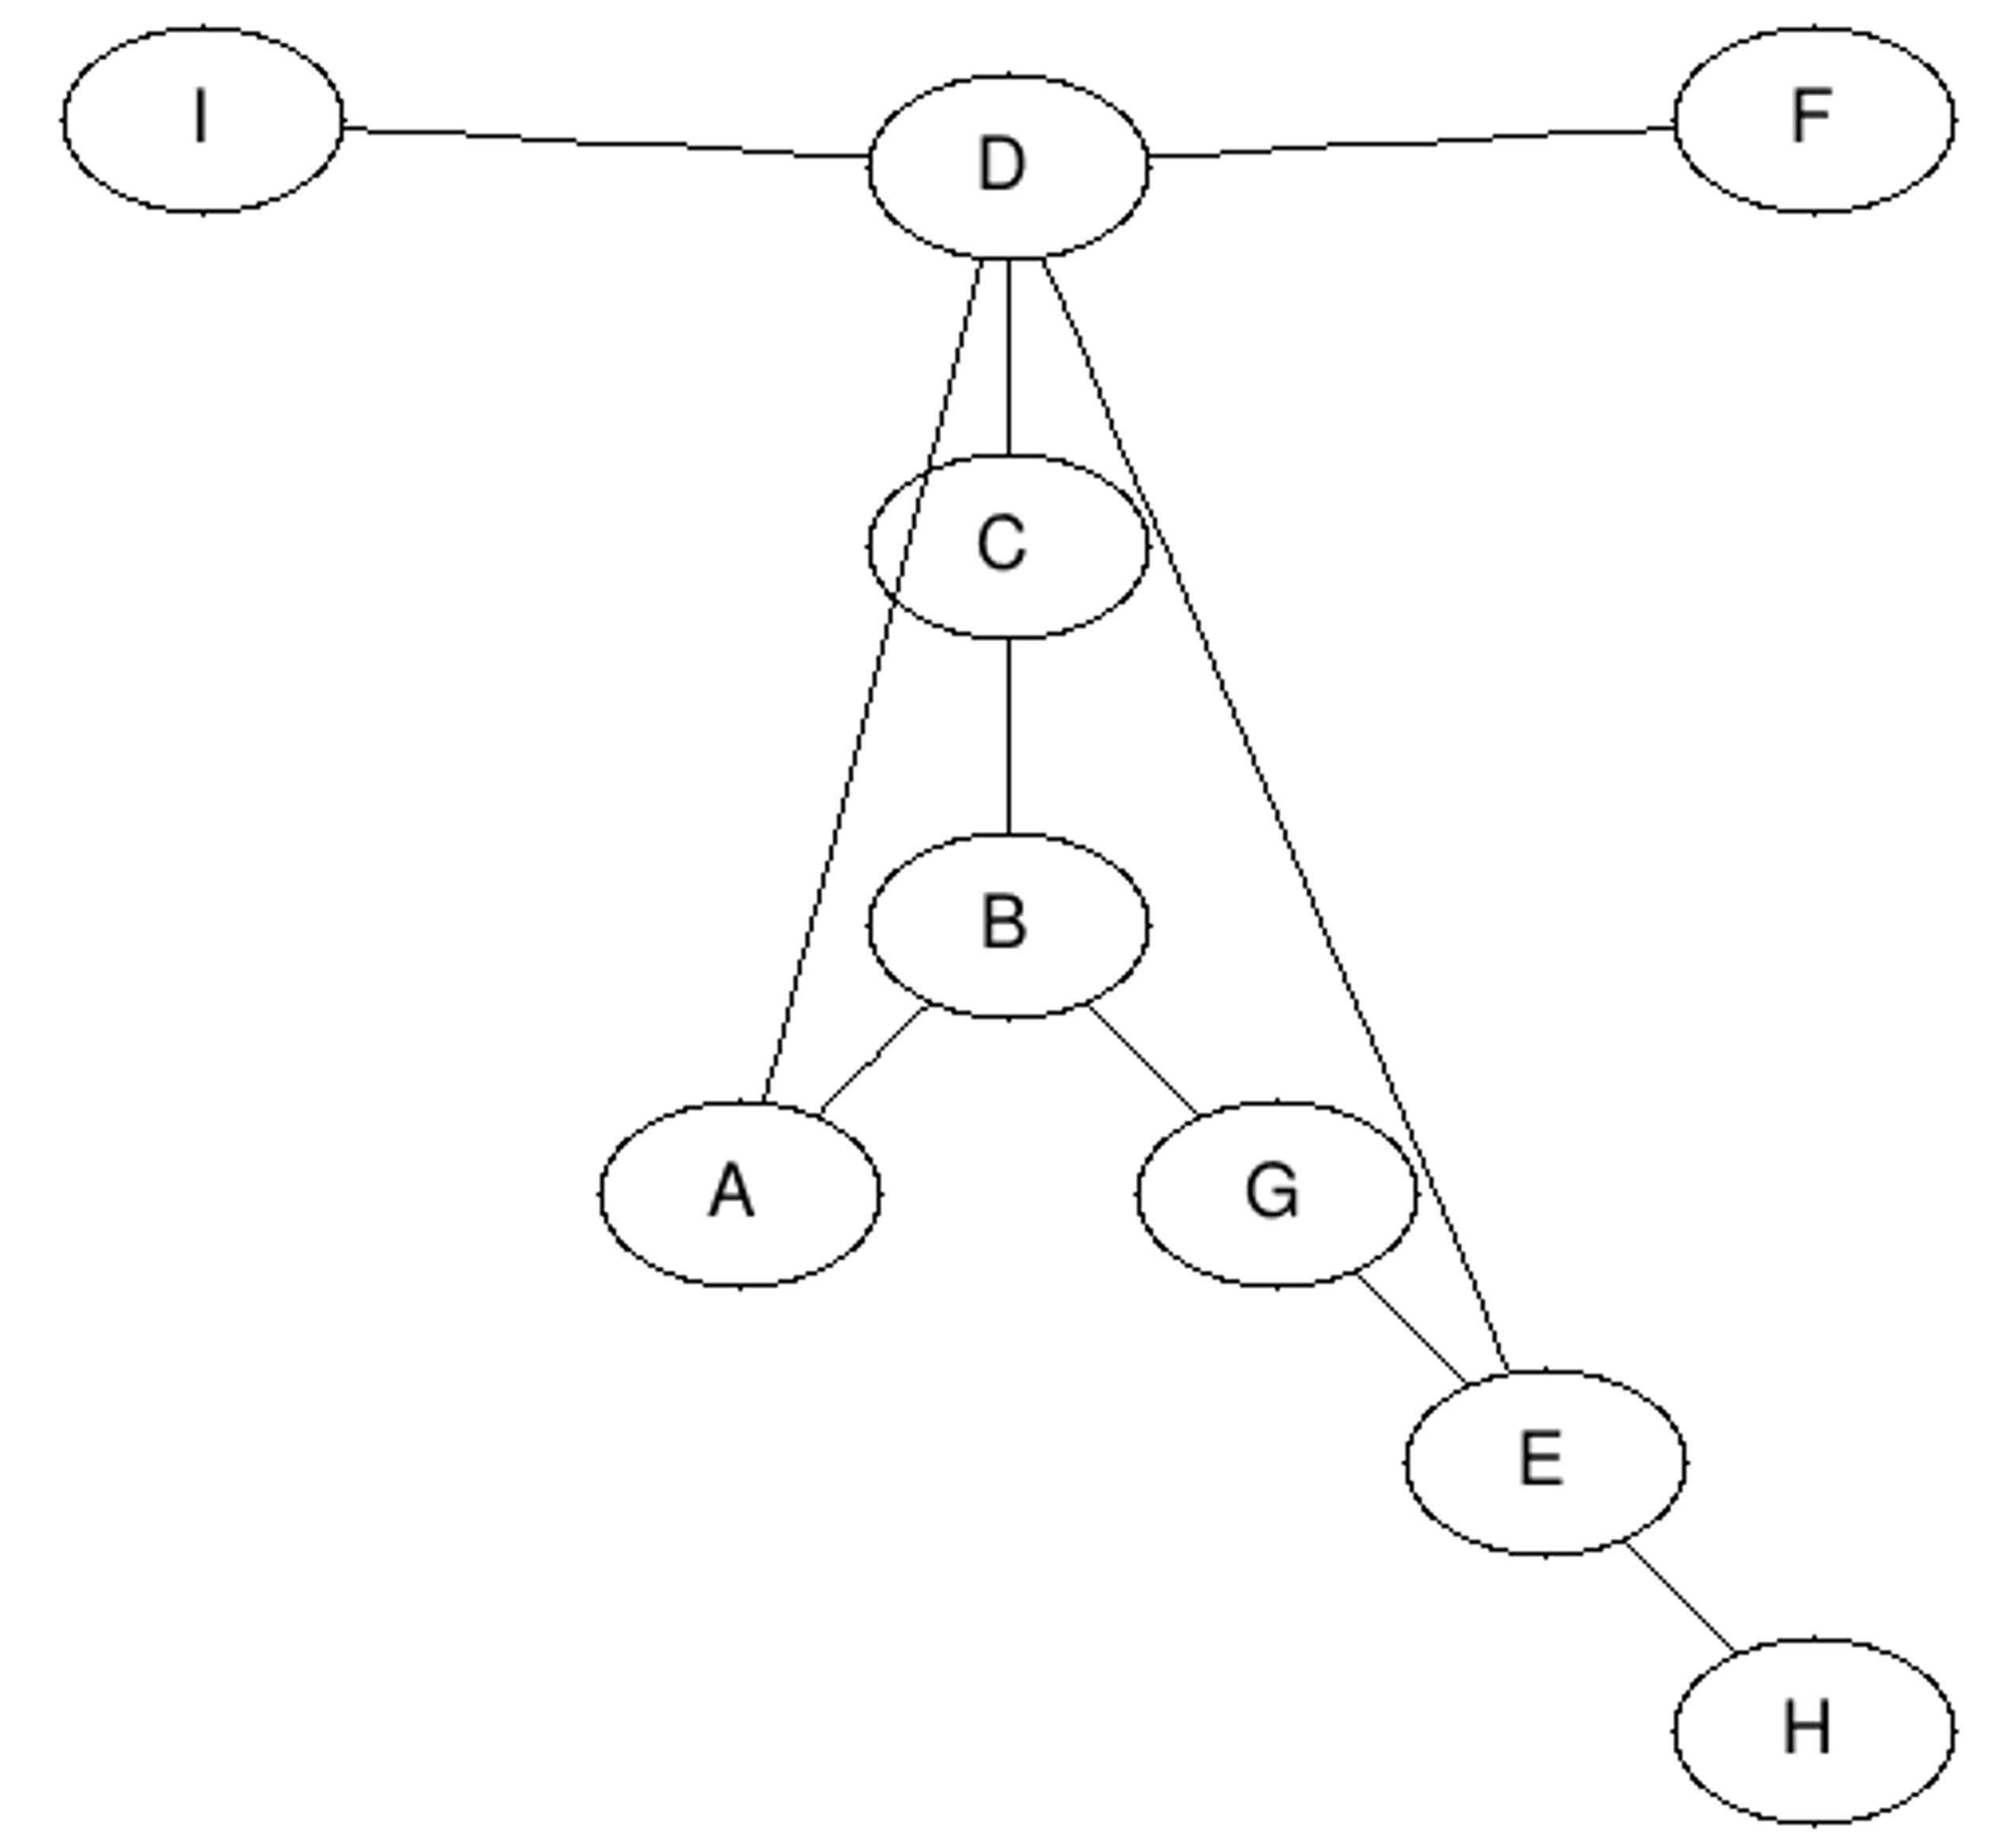
\includegraphics[width=0.6\textwidth]{pictures/twopi_example_2.png} 
\end{figure}

	Poslední rozložení je \uv{circo -- circular layout. This is suitable for certain diagrams of multiple cyclic structures, such as certain telecommunications networks.}\cite{graphviz_layout} 
	Jak už je zmíněno v~dokumentaci, grafy používající rozložení 
	circo se hodí jen k~nemnoha specifickým účelům. Jak vidíme na obrázku č.~3.6, opět se setkáváme s~nehierarchickým grafem. Algoritmus circo rozhodně má své využití, ale ne v~našem případě. V
	situaci, kdy připojujeme úložná zařízení v~systému Linux, se jen obtížně dostaneme do cyklických odkazů. Samotná podstata připojování úložných jednotek by měla zabraňovat těmto
	situacím. Pokud bychom už takovou situaci vytvořili, jedná se zcela určitě o~chybu buď používaných nástrojů, nebo chybu uživatelské konfigurace. 

\begin{figure}[h!]
	\label{Ukázka rozložení circo}
	\caption{Ukázka rozložení circo}
	\centering
	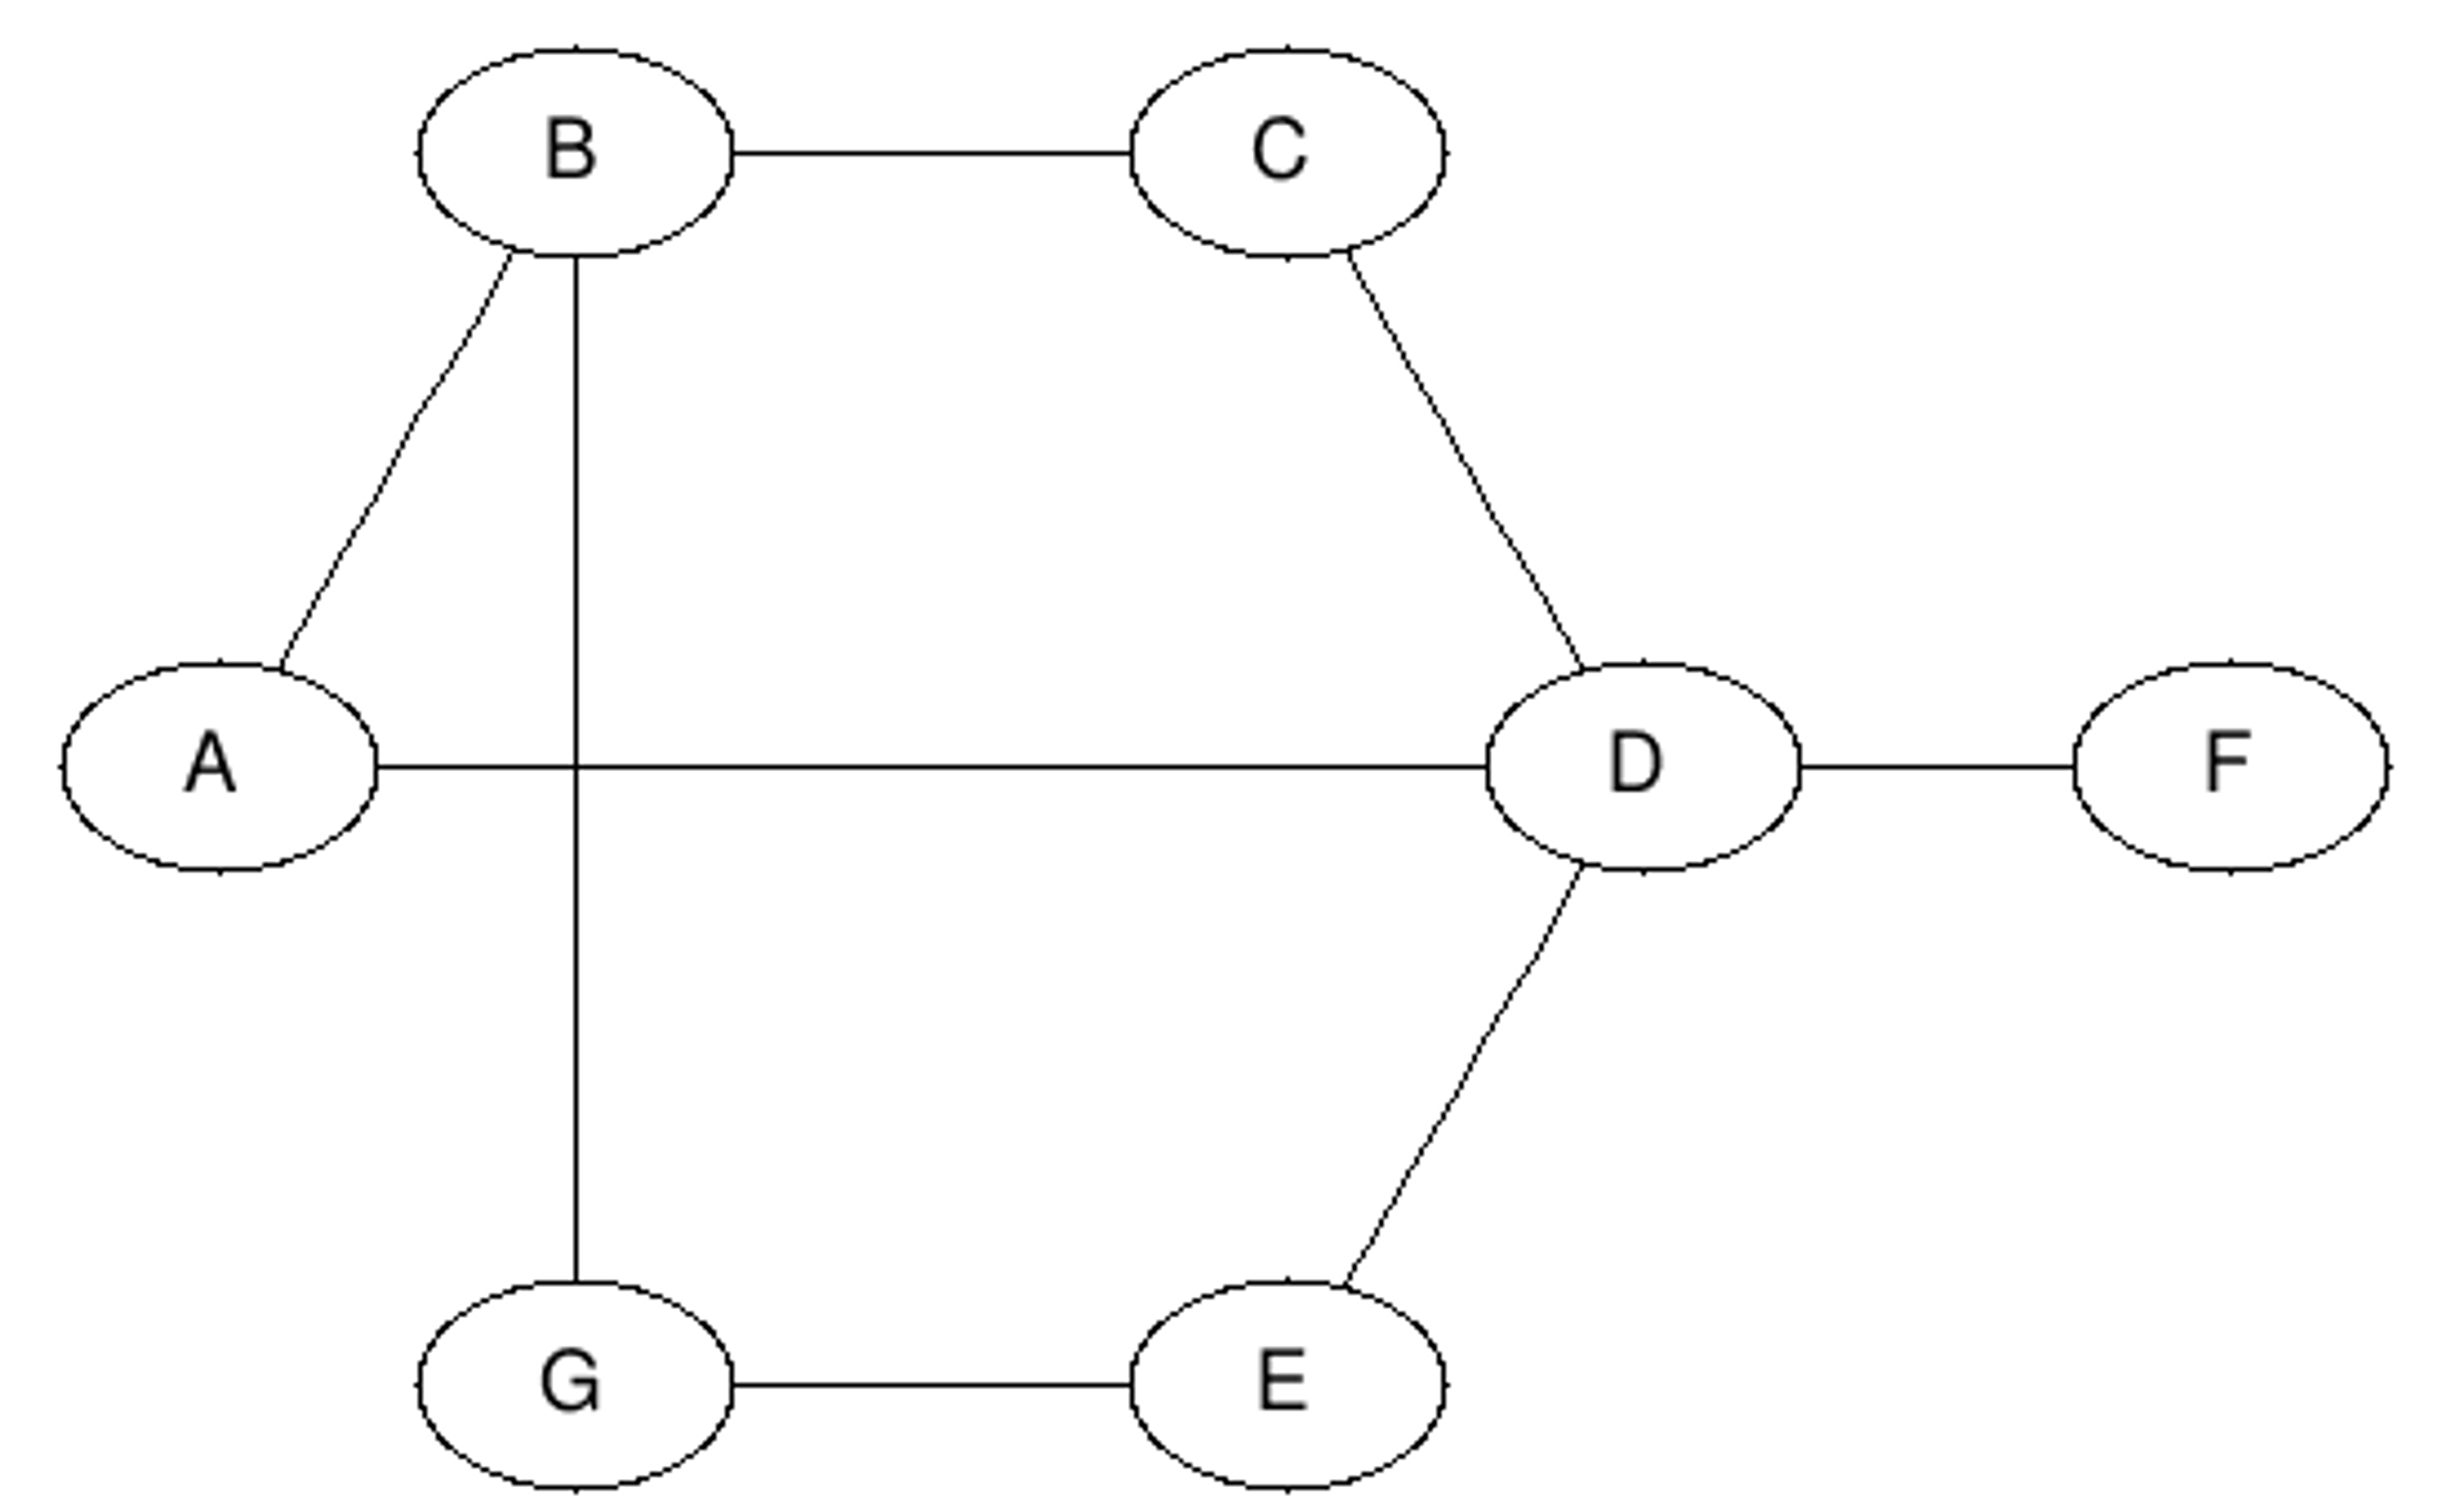
\includegraphics[width=0.6\textwidth]{pictures/circo_example.png} 
\end{figure}

	Algoritmem, který nakonec zbývá po aplikování vyřazovací metody, je algoritmus dot. 
	Základem pro mé rozhodnutí je stromová struktura. Ostatní typy rozložení nesplňují tuto podmínku, snad až na rozložení twopi. Twopi ale nelze použít kvůli větvení,
	ke kterému bude docházet velmi často. Navíc má problémy se dměma a~více kořenovými uzly, nezařazuje je k~sobě, pokud nejsou spojeny hranou. V~prostředí, kde je využívána technologie
	RAID, jde o~zcela nepřijatelnou vlastnost. Je potřebné, aby bloková zařízení logicky náležící k~sobě tak také byla vizualizována. Tuto podmínku splňuje
	jen dot. Není problém směrovat grafy 
	vytvářené rozložením dot shora dolů či zleva doprava, zmíněné chování lze nakonfigurovat. Tím odpadá poslední argument pro použití twopi, které na prvním příkladě graf situuje jako
	jdoucí zleva doprava.

\chapter{Aplikace}
	Aplikace je napsaná v~jazyce Python a~částečně využívá objektové paradigma. Důvody, které mě vedly k~výběru programovacího jazyka, jsou zmíněny v~úvodu práce. Objekty používám proto, že logicky
	dělí program do částí, ve kterých se snadno orientuje a~které spolu souvisí. Tak jsou rozděleny i~mé třídy. Třída pro načítání dat, pro tvorbu grafu, pro uzly, pro hrany atd.
	Za druhé, objektové programovaní je dnes de facto standardem a~velká část nově vznikajících programů používá jazyky, které podporují objektové programovaní. Za třetí,
	objektové programování usnadňuje spolupráci a~čtení kódu ostatními programátory. Jelikož rozšiřuji svobodný software, je pravděpodobné, že na něm někdo bude v~budoucnu pracovat
	a~rozšiřovat jej. Díky použití objektů bude mít usnadněnou práci.
	
\section{Třída \texttt{Visualiser}}
	Hlavní třída mého modulu je nazvaná \texttt{Visualizer}. Obsahuje základní atributy a~metody potřebné pro chod aplikace. Můžeme si ji představit jako centrální řídící jednotku. Ostatní
	třídy na ni navazují, ať už přímo nebo nepřímo (přes jinou třídu). 

	Třída Visualiser obsahuje seznam uzlů a~seznam hran. S~oběma seznamy pracují hlavně funkce v~jiných třídách. Nejdůležitější funkcí
	je funkce \texttt{create\_graph}. Její argumenty jsou jméno a~cesta ke grafu a~výsledkem je soubor SVG obsahující graf. 
	
	V~případě spouštění z~grafického rozhraní, si může uživatel v~okně aplikace vygenerovat graf, v~případě spuštění z~příkazové řádky jen uložit v~definovaném adresáři. 

	Třída obsahuje i~pomocnou funkci \texttt{prepare\_nodes}, která prochází jednotlivě uzly v~seznamu uzlů, a~nad každým spouští funkci \texttt{prepare}. Detailně funkci \texttt{prepare} rozebírám u~popisu uzlu.
	Pomocná funkce \texttt{prepare\_nodes}
	přemění data z~Blivetu na data vhodná pro Graphviz. Funkci jsem přidal do této třídy proto, že seznam uzlů je její atribut, a~i~funkce s~tímto atributem pracující by měla náležet do stejné třídy.

\section{Třída pro načítání dat}
	Třída pro načítání dat, \texttt{GvInput} slouží k~načítání dat z~Blivetu. Importuje Blivet jako modul a~vytvoří si instanci objektu obsahující veškeré informace
	o~blokových zařízeních. Verze knihovny Blivet 1.12.8, se kterou pracuji, vyžaduje před 
	každým načítáním dat spustit funkci \texttt{reset}. Tato funkce projde dostupné úložné kapacity a~vytvoří strom zařízení (\texttt{devicetree}). Stejně tak naplní seznam těmi
	samými objekty. Můj program prochází tento seznam (\texttt{Blivet.devices}) a~data z~něj si uloží do svých struktur. 
	
	V~případě že je instance objektu Blivet předána konstruktoru, se počítá s~tím, že má data připravena a~minimálně funkce \texttt{reset} byla zavolána.
	Ostatní kroky jsou totožné.

	Dalším krokem je vytvoření objektu reprezentujícho uzel grafu, jeho zpracování a~přidání do vlastního seznamu uzlů, který funguje jako převodník mezi Blivetem a~Graphvizem. Při
	přidávání do seznamu se uzly zároveň třídí pomocí přepínače a~jsou jim nastavovány barvy a~tvary. Vše, co potřebujeme pro zobrazení uzlu, se ukládá ihned při průchodu seznamem. 
	Tím dosáhneme nutnosti pouzejediného průchodu. Uzly si už pak informace zpracují samy. V~případě, že by uzel nebyl rozpoznán, nenastane situace kdy by program 
	havaroval. Jednoduše se při vytvoření použije přednastavená barva a~tvar (bílá, elipsa).

	Během zpracování vstupních dat je na
	standardní výstup vypsána hláška o~přidání nového členu seznamu. Uživatel tak má přehled, které uzly jsou přidány. Zařízení je identifikováno svým jménem a~typem.

	Po přidání uzlu se přidávají hrany. U~každého uzlu program projde seznam jeho rodičů a~vytvoří od nich hrany zpět k~právě vytvářenému uzlu. 
	Knihovna Blivet nemá jiné propojení mezi zařízeními než seznam rodičů. Stále ale stačí projít seznam zařízení jen jednou. Hrana se vytváří pomocí koncových uzlů, které má spojovat.
	Pokud jeden chybí, je vytvořen. Opět nedochází k~havárii programu. Pokud uzel existuje, je k~němu hrana připojena. Pokud uzel neexistuje, je později, až přijde na řadu, obarven.

\section{Třída \texttt{Node}}
	Třída pro uzly je poměrně jednoduchá, obsahuje převážně metody pro nastavení vzhledu. Nejdůležitější informace se ukládají už v~konstruktoru, jako ochrana opět slouží nastavení
	prázdných řetězců tam, kde by vstupní informace chyběly. Kromě konstruktoru obsahuje třída \texttt{Node} také funkce \texttt{change\_color} a~\texttt{change\_shape} nastavující vzhled. K~funkci 
	\texttt{change\_shape} 
	jsem vytvořil i~funkci \texttt{change\_style\_safely}. Pomáhá vytvořit styl uzlu se zakulacenými rohy. Graphviz řeší tuto situaci přidáním klíčového slova texttt{rounded} k~už 
	existujícímu stylu. Pokud je styl nastavený na obdélník s~ostrými rohy (box), je třeba přidat slovo rounded a~obě slova oddělit čárkou. Výsledek musí vypadat takto \uv{\texttt{box, rounded}},
	přičemž na pořadí slov nezáleží.

	Ukládání atributů a~\texttt{gv\_atributů} (atributů pro Graphviz) je řešeno pomocí slovníků. Použití slovníků umožňuje libovolně přidávat a~ubírat počty atributů. 
	Atributy rozumíme informace o~nastavení úložných zařízení, které se později vypisují ke každému uzlu. Jedinou výjimku tvoří jméno a~typ zařízení, neboť jde
	o~identifikační atributy a~jejich neexistence by znemožnila fungování programu. Rozhodl jsem se oddělit atributy pro knihovnu graphviz do samostatného slovníku. Díky tomu je při
	vykreslování grafu možné jen projít záznamy a~vytvořit z~párů klíč, hodnota páry atribut ulzu hodnota v~grafu. 

	Poslední pomocnou funkcí nacházející se v~tříde \texttt{Node} je fukce \texttt{prepare}. Připravuje textová data pro prezentaci ve formě grafu. Projde všechny záznamy ve slovníku \texttt{attributes} a~spojí je do 
	jednoho řetězce obsahujícího znaky nového řádku. Před spojením je možné flexibilně měnit počet a~obsah textových informací. Po spuštění funkce \texttt{prepare} jsou data uložena do štítku a~už není možné
	s~nimi manipulovat.

\section{Třída \texttt{Edge}}
	Třída pro hrany obsahuje konstruktor a~funkce pro získání počátečního a~koncového uzlu. Konstruktor bere za své argumenty právě tyto dvě 
	proměnné. Proměnnou \texttt{node\_from}, počáteční uzel a~proměnnou \texttt{node\_to}, koncový uzel. I~přesto, že neobsahuje mnoho funkcí, jsem se rozhodl vytvořit dedikovanou třídu pro hrany. 
	Takto je pro každý element v~grafu dedikovaná třída, se kterou lze pracovat při dalším možném rozšiřování mé práce.

\section{Třída pro vytváření grafů}
	Samotné vytváření grafu také není ničím zvlášť složitým, nicméně pro použití v~mé aplikaci je potřeba výsledný graf dále upravit. Rozeberme funkce ve ve třídě \texttt{Output} chronologicky
	tak, jak jsou použity. Tradičně konstruktor přebírá seznam uzlů a~hran. Volá funkci vytvářející graf se jménem \texttt{create\_gv\_graph} a~předává jí své argumenty. 

	Funkce \texttt{create\_gv\_graph} nejprve vytvoří orientovaný graf pomocí Graphvizu. Poté projde seznam uzlů a~pomocí graphvizu vytvoří všechny uzly v~nově utvořeném orientovaném grafu. Totéž udělá i
	s~hranami. Funkce pro vytváření uzlů \texttt{graphviz.node} bere jako první argument jméno uzlu. První argument je povinný, jméno uzlu. Povinný je argument jména
	i~při vytváření v~seznamu uzlů. Druhý argument ze tří je atribut \texttt{label}. Jde o~dlouhý řetězec rozdělený znaky dalších řádků, jak je vysvětleno výše v~částí věnující se třídě \texttt{Node}.
	Poslední argument je seznam zbylých atributů, které dokáže Graphviz zobrazovat. Je předán jako celý seznam a~po jeho rozbalení se aplikují nastavení vzhledu uzlu. Na konci je celý
	graf vrácen návratovou hodnotou.

	Druhá funkce se nazývá \texttt{create\_svg}. Jejím úkolem je přepsat graf do formátu SVG. Používá funkci \texttt{pipe} z~knihovny Graphviz. \texttt{Pipe} dokáže vytvářet i~jiné formáty, ale ty nejsou v~tuto
	chvíli důležité. Formát SVG byl vybrán proto, že v~něm lze použít JavaScript\cite{svg}, a~tím dosáhnout interaktivity. Konkrétně se jedná o~možnost zvětšovat uzly, posouvat a~přibližovat graf.
	Tuto funkcionalitu obstarává knihovna SVGPan\cite{svgpan}, uvolněná pod licencí BSD, je tedy možné ji zahrnout do jakéhokoliv programu.
	Popis funkcí následuje později, níže rozebírám postup implementace.

	Skript v~JavaScriptu vkládá pomocná funkce \texttt{insert\_JS\_to\_graph}, přebírající jeden argument, a~to řetězec obsahující SVG strukturu grafu, do kterého se má vložit zmíněný skript. 
	Kromě vložení JavaScriptu se funkce též stará o~drobné úpravy atributů SVG elementů tak aby JavaScript fungoval. 

\section{Třída \texttt{Gui}}
	Můj program lze používat jak dávkově z~příkazové řádky, tak interaktivně s~pomocí grafického uživatelského prostředí. Dávkový režim nabízí pouze možnost vygenerovat graf v~určitém 
	umístění. Interaktivní režim nabízí možnost graf prohlížet. Variací na interaktivní režim je také okno s~grafem, které by se mohlo zobrazit při instalaci, jako vizualizace změn prováděných
	instalátorem. Třída \texttt{Gui} též obsahuje funkci \texttt{show}, která slouží pro otevření okna a~okamžitému zobrazení vygenerovaného grafu. 
	Při integraci mého programu do programu Blivet-gui bude dostačující volat tyto dvě funkce a~zbytek zařídí můj vizualizační program.

	Třída \texttt{Gui} obsahuje vše potřebné pro obsluhu uživatelského rozhraní. Je naprogramována s~pomocí nejrozšířenější linuxové knihovny pro uživatelská rozhraní Gnome toolkit (GTK). Jde o~
	obyčejné okno s~několika tlačítky. Jsou v~ní obsaženy ovládací prvky potřebné pro nastavení umístění grafu, tlačítko pro vyvolání kontextové
	nápovědy a~plocha zobrazující samotný graf. Pro zobrazení grafu je použita technologie WebKit. WebKit je de facto prohlížeč, který je možné vložit do GTK aplikace.
	Okno WebKitu je možné vložit do GTK aplikace a~tím dosáhnout stejné základní funkcionality,
	jakou mají dnešní moderní webové prohlížeče. V~mém případě jde o~schopnost zobrazit SVG a~schopnost spouštět JavaScript.

	Rizikem, které je nutné přijmout, je možná známá zranitelnost prohlížečů a~nutnost ukládat soubor SVG na disku. WebKit totiž zobrazuje SVG s~pomocí protokolu \texttt{file://}. Počítač se
	tak ptá sám sebe na existenci souboru v~určité cestě definované uživatelem, a~pokud jej najde, zobrazí jej uživateli. Pokud by se k~systému dostal útočník, mohl by soubor upravit a~
	zanechat v~něm škodlivý kód. Nicméně bezpečnost systému není věcí této práce a~vychází se z~předpokladu, že systém, na kterém je vizualizace spouštěna, je buď ve fázi instalace, nebo
	je již zabezpečen. 

\chapter{Vzhled grafu}
  Můžeme uvažovat o~třech hlavních způsobech uložení informací v~grafu. První je ve formě textu, druhá ve formě vzhledu uzlů a~třetí ve formě obrázků 
	u~některých druhů blokových zařízení. 

	Při vygenerování grafu však nejsou všechna data ihned zobrazena, některé informace jsou skryté a~ostatní zvýrazněné. Uzly jsou klikatelné a~po kliknutí
	se uzel zvětší a~zároveň se zobrazí kompletní informace. Po opětovném klikutí je uzel uveden do předchozího stavu, tj. zmenšen a~informace jsou částečně 
	skryty. Ve zmenšeném stavu jsou taktéž zvýrazněny zbylé řádky. Díky tomu je graf přehlednější a~zároveň je možné zjistit o~každém uzlu dostatek informací.

\section{Textové informace}
  Převážná většina informací je uložena ve formě textu. Jednotlivé atributy blokových zařízení jsou uspořádáy do řádků a~vloženy do uzlu. Výběr velikosti
	písma a~fontu je přenechán programu Graphviz. První je uvedeno jméno zařízení, následované jeho typem a~formátem. Dále jsou přidány další řádky, 
	obsahující dodatečné informace. Jméno, typ a~formát jsou řádky zvýrazněné pomocí JavaScriptu, neboť rozpoznání, jaké zařízení daný uzel reprezentuje.

	Dále jsou uvedeny informace, které jsou nutné pro přehled o~zařízeních, ale nejsou nutné pro rozeznání uzlů. Jde o~informace o~velikosti blokového
	zařízení, různé identifikátory a~adresářová cesta k~umístění zařízení. V~případě, že se jedná o~graf reprezentující chystané akce, které jsou připravené
	k~provedení, je u~každého dotčeného uzlu uvedeno, jaké akce jsou s~ním naplánované. Naplánovaných akcí může být i~více než jedna, v~tom případě jsou
	řazeny za sebe na stejný řádek. Například při změně formátu je nejdříve starý formát zničen a~poté je nový formát vytvořen, jde tedy o~dvě akce a~
	uživatel je o~obou informován.

  Na obrázku č.~5.1 je vidět rozdíl mezi přiblíženým a~nepřiblíženým uzlem. Rozdíl ve velikosti písma není markantní, spíše si lze všimnout rozdílu ve velikosti 
	uzlu.

\begin{figure}[]
	\label{fig:Rozdíly uzlů}
	\caption{Vlevo přiblížený graf v~pravo nepřiblížený}
	\centering
	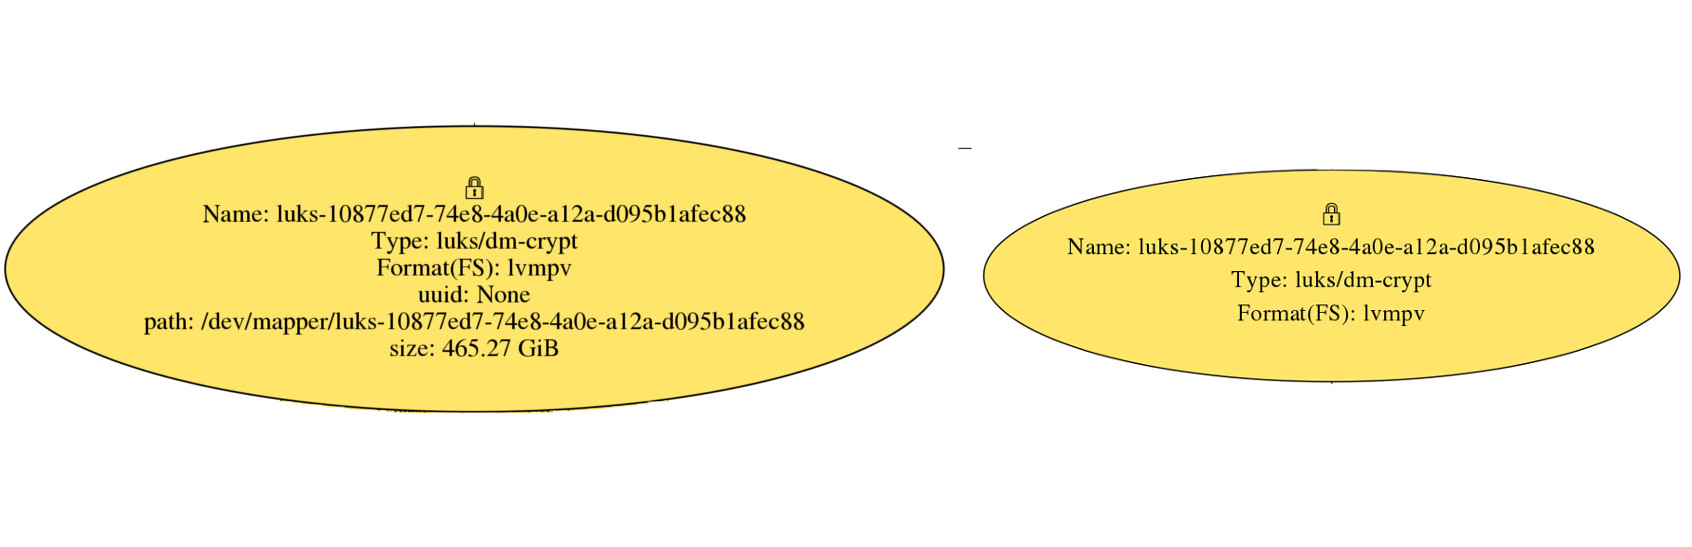
\includegraphics[width=1.0\columnwidth]{pictures/node_zoom.jpg}
\end{figure}
  
\section{Netextové informace}
  Informace jsou kromě textu uloženy též ve formě vzhledu uzlů. Kromě hierarchie uzlů to je jejich barva a~tvar. Fyzické disky a~jejich oddíly jsou
	reprezentovány obdélníkem, naopak šifrování a~RAID jsou reprezentovány
	elipsou. Idea je taková, že čím je objekt reprezentovaný uzlem abstraktnější, tím je uzel zaoblenější. Existuje i~mezistupeň obdélníku se zaoblenými
	rohy, jakožto i~jiné použité tvary. Na obrázku č.~5.2 uvádím příklad fyzického disku vlevo a~šifrování technologií LUKS vpravo.
\begin{figure}[h!]
	\label{fig:Rozdíly zařízení}
	\caption{Ukázka rozdílné reprezentace různých zařízení}
	\centering
	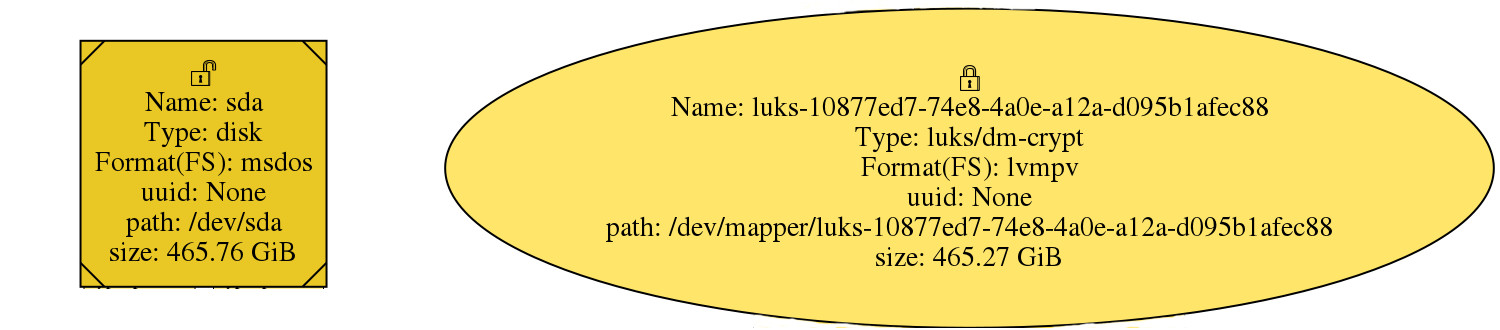
\includegraphics[width=.9\columnwidth]{pictures/disk_and_luks.jpg}
\end{figure}

	Druhým vodítkem je barva, respektive odstíny jedné barvy. Opět platí čím abstraktnější blokové zařízení, tím světlejší barva . Dále využívám
	barvy na odlišení různých akcí, které byly naplánované předem. Akce, u~kterých dochází ke smazaní zařízení, jsou zobrazeny červeně. Naproti tomu akce,
	u~kterých je zařízení vytvořeno, jsou zobrazeny zeleně. Při akcích typu formátování, zvětšení či zmenšení oddílu je barva modrá. Příklady jsou uvedeny na obrázku č.~5.3.

\begin{figure}
	\label{fig:Reprezentace naplánované akce}
	\caption{Ukázky reprezentace akcí}
	\centering
	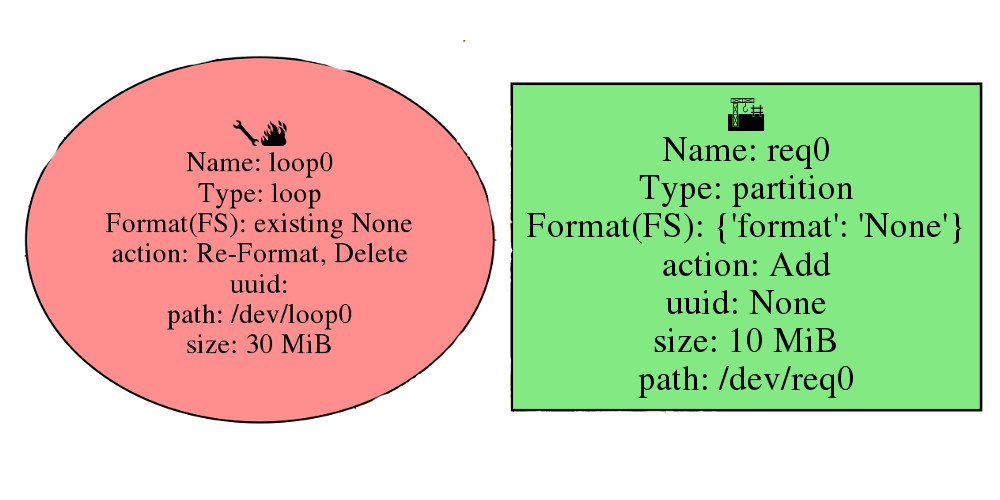
\includegraphics[width=.9\columnwidth]{pictures/actions.jpg}
\end{figure}
  
\section{Informace předávané symboly -- emoji}
  Informace jsou uchovávané také v~podobě malých symbolů známých pod jménem emoji, které můžeme vidět na obrázcích č.~5.2 a~5.3.
	Původně vznikly v~Japonsku jako rozšíření emotikonů. Internetem se pak rozšířily do
	celého světa. Dnes jsou již zahrnuty do standardní znakové sady Unicode\cite{emoji}. Nicméně to neznamená, že jsou na všech platformách všechny znaky standardizované.  Ve své práci používám několik základních symbolů, které 
	jsou součástí standardní sady Unicode, a~proto by měly být podporovány všude.

  Jak je vidět na obrázku č.~5.3, symboly jsou použity pro rychlejší rozpoznání, které akce jsou připravené. Barva uzlu je jen jedna, ale emoji symbolů může být u~jednoho uzlu i~více. Symboly jsou
	zobrazované na vrchu uzlu ještě před jménem. Z~hlediska dostupných možností to byla nejlepší volba. Uvažoval jsem i~o~možnosti uzel rozdělit na textovou a~obrázkovou část a~zobrazovat
	oba typy dat odděleně, ale kvůli limitům Graphvizu jsem zvolil umístění na vrchu uzlu.

\chapter{Závěr}
  Hlavními cíli mé byla vizualizace dat z~Blivetu do samostatného okna GTK aplikace a~zobrazení připravených změn. Stejně tak jsou připraveny funkce pro snadnou integraci
	do dalších programů.   

	Vizualizační program čte data z~knihovny Blivet a~s~pomocí knihovny Graphviz z~nich vytváří graf. Ten zobrazuje s~pomocí programu WebKit ve vlastním okně aplikace. Program lze
	použít také k~vytvoření grafu bez jeho zobrazení. Grafy se dělí na dva druhy, graf se zvýrazněním naplánovaných akcí a~bez něj.

	Se zobrazeným grafem je možno manipulovat pomocí JavaScrip\-tu\cite{javascript}, graf je možno posouvat a~přibližovat. JavaScript také zajišťuje funkci \uv{rozklikávání} uzlů. Přiblížené uzly zobrazují
	více informací, nepřiblížené zpřehledňují graf.

	Na výsledek mé práce je možné dále navázat.
	Prvním rozšířením je funkcionalita zajišťující schopnost vytvářet soubory XML obsahující informace z~grafů. 
	Již existuje aplikace schopná vytvářet soubory XML z~Blivetu a~zase je nahrávat zpět. Její zamýšlené
	použití je vytváření záchytných bodů, ke kterým je možné se vrátit v~případě havárie instalátoru, přerušení dodávky elektrického proudu či jiné fatální chyby systému. Ideou pro export
	XML z~grafu je možnost na systém přenést tu konfiguraci, která je prezentována na grafu přes soubor XML.

	Druhým a~ambicióznějším rozšířením je schopnost grafu fungovat jako samostatný konfigurační nástroj. Graf by nejenom zobrazoval data, která mu byla poskytnuta, ale také by je byl
	schopen upravovat a~předávat nová data zpět aplikaci Blivet, popřípadě instalátoru. Například by bylo možné přesouvat logické oddíly LVM (logical volume
	management) mezi PV (physical volume) jednoduchým 
	přetažením myší stejně, jako dnes kopírujeme soubory přetažením jejich ikony. Nové oddíly by byly vytvářeny také přetažením z~nějaké nabídky předpřipravených uzlů. Konkrétní velikosti
	a~jména zařízení by se editovaly pomocí textových polí v~každém uzlu.
	
	Největším problémem, který by bylo třeba vyřešit, je načítání SVG a~informací z~něj zpět zároveň s~ukládáním informací z~prohlížeče. 
	Jedním z~možných postupů by byla úprava XML načítače tak, aby fungoval i~pro SVG graf zobrazovaný uživateli. Uživatel by přetvořil graf podle svých představ, poté spustil 
	konfiguraci, a~ta by přenesla stav do Blivetu a~provedla změny v~úložném prostoru systému. 

	\printbibliography

\end{document}
